% {{{ Preamble ----------------------------------------------------------------
\documentclass{beamer}

% encodings, fonts etc.
\usepackage[utf8x]{inputenc}
\usepackage[T1]{fontenc}

% Hold kæft utf
\makeatletter
\def\UTFviii@defined#1{%
  \ifx#1\relax
      ?%
  \else\expandafter
    #1%
  \fi
}

\makeatother

% math packages
\usepackage{amsmath, amssymb, amsthm}
\usepackage{mathtools}

% beamer configuration
\usetheme{Copenhagen}
%\useoutertheme{infolines}
%\usetheme{metropolis}
\beamertemplatenavigationsymbolsempty
%\setbeamertemplate{theorems}[numbered]
\setbeamersize{description width=2.0em}

%\usepackage{pgfpages}
%\setbeameroption{show notes}
%\setbeameroption{show notes on second screen=right}

% algorithms
\usepackage{algorithm}
\usepackage[noend]{algpseudocode}

% misc. packages
\usepackage{float}
\usepackage{varwidth}
\usepackage{listings}
\lstset{
  %breaklines=true,
  keepspaces=true,
  %frame=ltrb,
  %framesep=1pt,
  %commentstyle=\color{grey},
  basicstyle=\ttfamily\tiny,
  %numbers=left,
  title=\lstname,
  %columns=fullflexible,
  inputencoding=utf8,
  extendedchars=true,
}

% graphics and tikz
\usepackage{pgf}
\usepackage{tikz}
\usetikzlibrary{positioning,arrows,calc}
\tikzset{
    on grid,
    node distance=3cm,
    auto,
    block/.style = {
        draw,
        shape=rectangle,
        minimum height=3em,
        minimum width=3em,
        line width=1pt
    },
    control/.style = {
        draw,
        shape=circle,
        minimum height=7em,
        minimum width=3em,
        line width=1pt
    },
    mux/.style = {
        draw,
        shape=rectangle,
        minimum height=1.5em,
        minimum width=1em,
        line width=1pt
    },
    empty/.style = {
        shape=rectangle,
        minimum height=3em,
        minimum width=3em
    },
    >=latex',
}


% mathematics
\newtheorem{proposition}{Proposition}

\renewcommand{\tt}{\texttt}

% title page
\title{Core Components}
\author[Carl-Johannes Johnsen]{
  \mbox{Carl-Johannes Johnsen}}
\institute{Department of Computer Science\\
           University of Copenhagen}
%\date{December 22, 2016}
% }}} -------------------------------------------------------------------------

\begin{document}

% {{{ Title page --------------------------------------------------------------
\frame{\titlepage}
% }}} -------------------------------------------------------------------------

% {{{ Table of contents -------------------------------------------------------
%\begin{frame}
%  \frametitle{Outline}
%  \tableofcontents
%\end{frame}
% }}} -------------------------------------------------------------------------

\section{Introduction}
\begin{frame}
    In this lecture, we will be looking at the major components of the MIPS
    processor.

    \vspace{\baselineskip}
    By combining these components, we should be able to construct a single
    cycle MIPS processor.
\end{frame}
\subsection{Overview of the processor}
\begin{frame}
    \begin{figure}
        \centering
        \scalebox{0.5}{
            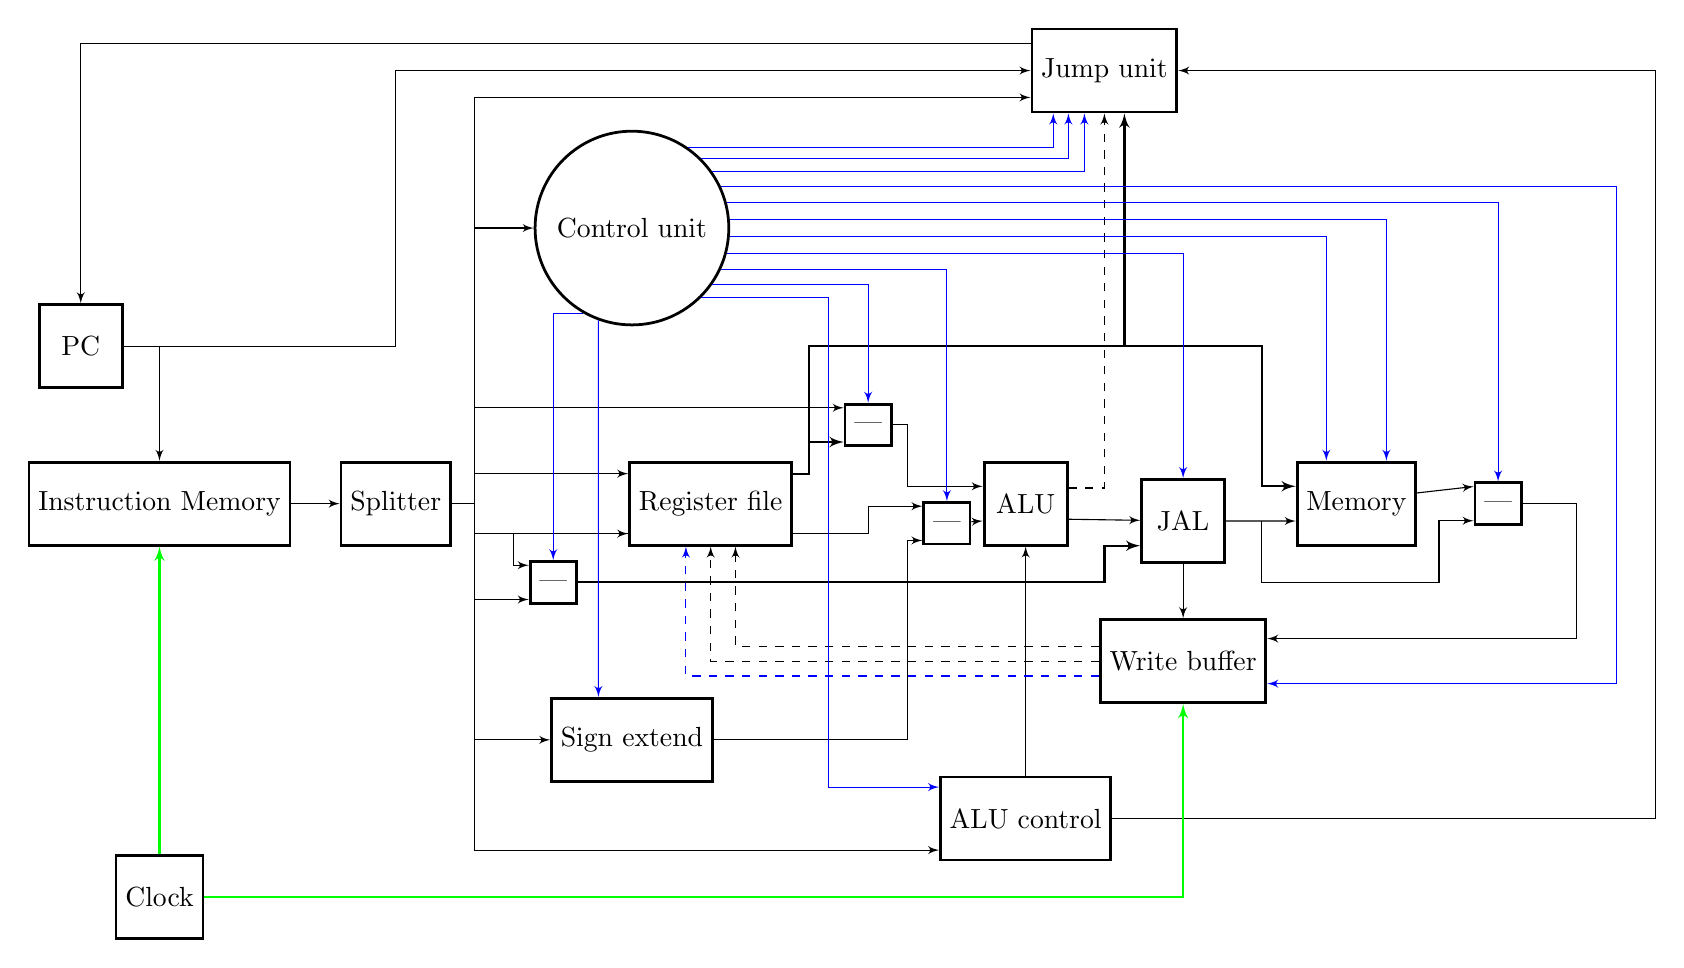
\begin{tikzpicture}
                \node[block] (reg) at (0,0) {Register file};
                \node[control] (cont) at (-1,3.5) {Control unit};
                \node[block] (jump) at (5,5.5) {Jump unit};
                \node[empty] (splitspace) at (-3,0) {};
                \node[block] (split) at (-4,0) {Splitter};
                \node[block] (if) at (-7,0) {Instruction Memory};
                \node[block] (sign) at (-1,-3) {Sign extend};
                \node[block] (alu) at (4,0) {ALU};
                \node[block] (alucont) at (4,-4) {ALU control};
                \node[block] (mem) at (8.2,0) {Memory};
                \node[block] (jal) at (6,-0.22) {JAL};
                \node[mux] (memread) at (10,0) {|};
                \node[mux] (shmt) at (2,1) {|};
                \node[mux] (imm) at (3, -0.25) {|};
                \node[mux] (regdst) at (-2,-1) {|};
                \node[block] (pc) at (-8, 2) {PC};
                \node[block] (writebuf) at (6, -2) {Write buffer};

                \path[draw, ->] (if) -- (split);
                \path[draw, -] (split) -- (splitspace.center);
                \path[draw, ->] (splitspace.center) |- (sign);
                \path[draw, ->] (splitspace.center) |- (cont);
                \path[draw, ->] (splitspace.center) |- (reg.160);
                \path[draw, ->] (splitspace.center) |- (reg.200);
                \path[draw, ->] (splitspace.center) |- (jump.200);
                \path[draw, ->] (splitspace.center) |- (alucont.200);
                \path[draw, ->] (splitspace.center) |- (regdst.215);
                \path[draw, ->] (splitspace.center) |- (shmt.145);
                \path[draw, ->] (reg.200) -| (-2.5, -0.5) |- (regdst.145);
                \path[draw, ->] (alucont) -- (alu);
                \path[draw, ->] (alucont) -| (12, 0) |- (jump);
                \path[draw, ->] (reg.340) -| (2,-0.25) |- (imm.145);
                \path[draw, thick, ->] (reg.20) -| (1.25,0.5) |- (shmt.215);
                \path[draw, thick, ->] (1.25, 0.5) |- (4, 2) -| (7,1) |- (mem.164);
                \path[draw, thick, ->] (4,2) -| (jump.295);
                \path[draw, ->] (shmt) -| (2.5, 0.5) |- (alu.158);
                \path[draw, dashed, ->] (alu.20) -| (jump);
                \path[draw, ->] (alu.340) -- (jal);
                \path[draw, ->] (jal) -- (mem.196);
                \path[draw, ->] (imm) -- (alu.202);
                \path[draw, ->] (7, -0.22) |- (8, -1) -| (9.25,-0.5) |-
                (memread.215);
                \path[draw, ->] (mem.10) -- (memread.145);
                \path[draw, ->] (sign) -| (2.5, -1) |- (imm.215);
                \path[draw, thick, ->] (regdst) -| (5, -0.6) |- (jal.210);
                \path[draw, ->] (pc) -| (if);
                \path[draw, ->] (pc) -| (-4, 4) |- (jump);
                \path[draw, ->] (jump.160) -| (pc);
                \path[draw, ->] (jal) -- (writebuf);
                \path[draw, ->] (memread) -| (11, -1) |- (writebuf.15);
                \path[draw, dashed, ->] (writebuf.170) -| (reg.300);
                \path[draw, dashed, ->] (writebuf) -| (reg);
                \path[draw, dashed, ->, color=blue] (writebuf.190) -| (reg.240);

                \path[draw, ->, color=blue] (cont.55) -| (jump.220);
                \path[draw, ->, color=blue] (cont.45) -| (jump.230);
                \path[draw, ->, color=blue] (cont.35) -| (jump.245);
                \path[draw, ->, color=blue] (cont.25) -| (11.5,0) |-
                (writebuf.345);
                \path[draw, ->, color=blue] (cont.15) -| (memread);
                \path[draw, ->, color=blue] (cont.5) -| (mem.55);
                \path[draw, ->, color=blue] (cont.355) -| (mem.125);
                \path[draw, ->, color=blue] (cont.345) -| (jal);
                \path[draw, ->, color=blue] (cont.335) -| (imm);
                \path[draw, ->, color=blue] (cont.325) -| (shmt);
                \path[draw, ->, color=blue] (cont.315) -| (1.5, 0.5) |-
                (alucont.160);
                %\path[draw, ->, color=blue] (cont.315) -- (reg.95);
                %\path[draw, ->, color=blue] (cont.305) -- (reg.110);
                \path[draw, ->, color=blue] (cont.250) -- (sign.128);
                \path[draw, ->, color=blue] (cont.240) -| (regdst);

                \node[block] (clock) at (-7, -5) {Clock};
                \path[draw, ->, thick, color=green] (clock) -- (if);
                \path[draw, ->, thick, color=green] (clock) -| (writebuf);
            \end{tikzpicture}
        }
    \end{figure}
\end{frame}
\begin{frame}
    \begin{figure}
        \centering
        \scalebox{0.5}{
            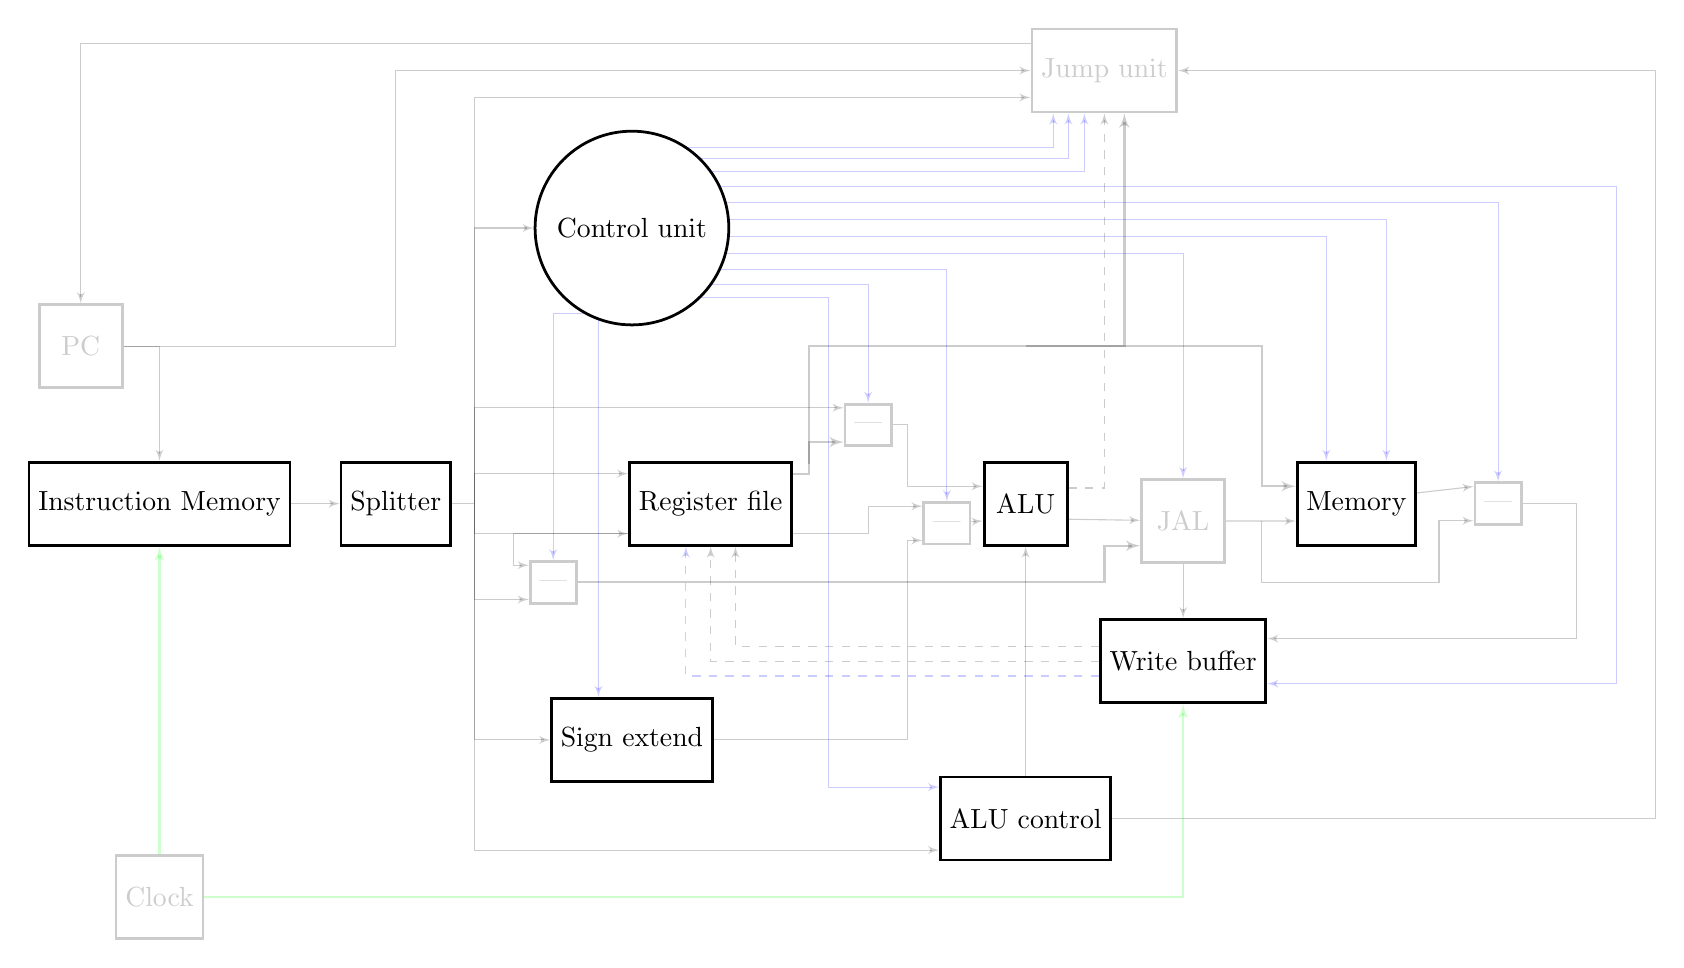
\begin{tikzpicture}
                \node[block] (reg) at (0,0) {Register file};
                \node[control] (cont) at (-1,3.5) {Control unit};
                \node[opacity=0.2,block] (jump) at (5,5.5) {Jump unit};
                \node[opacity=0.2,empty] (splitspace) at (-3,0) {};
                \node[block] (split) at (-4,0) {Splitter};
                \node[block] (if) at (-7,0) {Instruction Memory};
                \node[block] (sign) at (-1,-3) {Sign extend};
                \node[block] (alu) at (4,0) {ALU};
                \node[block] (alucont) at (4,-4) {ALU control};
                \node[block] (mem) at (8.2,0) {Memory};
                \node[opacity=0.2,block] (jal) at (6,-0.22) {JAL};
                \node[opacity=0.2,mux] (memread) at (10,0) {|};
                \node[opacity=0.2,mux] (shmt) at (2,1) {|};
                \node[opacity=0.2,mux] (imm) at (3, -0.25) {|};
                \node[opacity=0.2,mux] (regdst) at (-2,-1) {|};
                \node[opacity=0.2,block] (pc) at (-8, 2) {PC};
                \node[block] (writebuf) at (6, -2) {Write buffer};

                \path[opacity=0.2,draw, ->] (if) -- (split);
                \path[opacity=0.2,draw, -] (split) -- (splitspace.center);
                \path[opacity=0.2,draw, ->] (splitspace.center) |- (sign);
                \path[opacity=0.2,draw, ->] (splitspace.center) |- (cont);
                \path[opacity=0.2,draw, ->] (splitspace.center) |- (reg.160);
                \path[opacity=0.2,draw, ->] (splitspace.center) |- (reg.200);
                \path[opacity=0.2,draw, ->] (splitspace.center) |- (jump.200);
                \path[opacity=0.2,draw, ->] (splitspace.center) |- (alucont.200);
                \path[opacity=0.2,draw, ->] (splitspace.center) |- (regdst.215);
                \path[opacity=0.2,draw, ->] (splitspace.center) |- (shmt.145);
                \path[opacity=0.2,draw, ->] (reg.200) -| (-2.5, -0.5) |- (regdst.145);
                \path[opacity=0.2,draw, ->] (alucont) -- (alu);
                \path[opacity=0.2,draw, ->] (alucont) -| (12, 0) |- (jump);
                \path[opacity=0.2,draw, ->] (reg.340) -| (2,-0.25) |- (imm.145);
                \path[opacity=0.2,draw, thick, ->] (reg.20) -| (1.25,0.5) |- (shmt.215);
                \path[opacity=0.2,draw, thick, ->] (1.25, 0.5) |- (4, 2) -| (7,1) |- (mem.164);
                \path[opacity=0.2,draw, thick, ->] (4,2) -| (jump.295);
                \path[opacity=0.2,draw, ->] (shmt) -| (2.5, 0.5) |- (alu.158);
                \path[opacity=0.2,draw, dashed, ->] (alu.20) -| (jump);
                \path[opacity=0.2,draw, ->] (alu.340) -- (jal);
                \path[opacity=0.2,draw, ->] (jal) -- (mem.196);
                \path[opacity=0.2,draw, ->] (imm) -- (alu.202);
                \path[opacity=0.2,draw, ->] (7, -0.22) |- (8, -1) -| (9.25,-0.5) |- (memread.215);
                \path[opacity=0.2,draw, ->] (mem.10) -- (memread.145);
                \path[opacity=0.2,draw, ->] (sign) -| (2.5, -1) |- (imm.215);
                \path[opacity=0.2,draw, thick, ->] (regdst) -| (5, -0.6) |- (jal.210);
                \path[opacity=0.2,draw, ->] (pc) -| (if);
                \path[opacity=0.2,draw, ->] (pc) -| (-4, 4) |- (jump);
                \path[opacity=0.2,draw, ->] (jump.160) -| (pc);
                \path[opacity=0.2,draw, ->] (jal) -- (writebuf);
                \path[opacity=0.2,draw, ->] (memread) -| (11, -1) |- (writebuf.15);
                \path[opacity=0.2,draw, dashed, ->] (writebuf.170) -| (reg.300);
                \path[opacity=0.2,draw, dashed, ->] (writebuf) -| (reg);
                \path[opacity=0.2,draw, dashed, ->, color=blue] (writebuf.190) -| (reg.240);

                \path[opacity=0.2,draw, ->, color=blue] (cont.55) -| (jump.220);
                \path[opacity=0.2,draw, ->, color=blue] (cont.45) -| (jump.230);
                \path[opacity=0.2,draw, ->, color=blue] (cont.35) -| (jump.245);
                \path[opacity=0.2,draw, ->, color=blue] (cont.25) -| (11.5,0) |-(writebuf.345);
                \path[opacity=0.2,draw, ->, color=blue] (cont.15) -| (memread);
                \path[opacity=0.2,draw, ->, color=blue] (cont.5) -| (mem.55);
                \path[opacity=0.2,draw, ->, color=blue] (cont.355) -| (mem.125);
                \path[opacity=0.2,draw, ->, color=blue] (cont.345) -| (jal);
                \path[opacity=0.2,draw, ->, color=blue] (cont.335) -| (imm);
                \path[opacity=0.2,draw, ->, color=blue] (cont.325) -| (shmt);
                \path[opacity=0.2,draw, ->, color=blue] (cont.315) -| (1.5, 0.5) |- (alucont.160);
                %\path[opacity=0.2,draw, ->, color=blue] (cont.305) -- (reg.110);
                \path[opacity=0.2,draw, ->, color=blue] (cont.250) -- (sign.128);
                \path[opacity=0.2,draw, ->, color=blue] (cont.240) -| (regdst);

                \node[opacity=0.2,block] (clock) at (-7, -5) {Clock};
                \path[opacity=0.2,draw, ->, thick, color=green] (clock) -- (if);
                \path[opacity=0.2,draw, ->, thick, color=green] (clock) -| (writebuf);
            \end{tikzpicture}
        }
    \end{figure}
\end{frame}
\section{Register File}
\begin{frame}
    \begin{figure}
        \centering
        \scalebox{0.5}{
            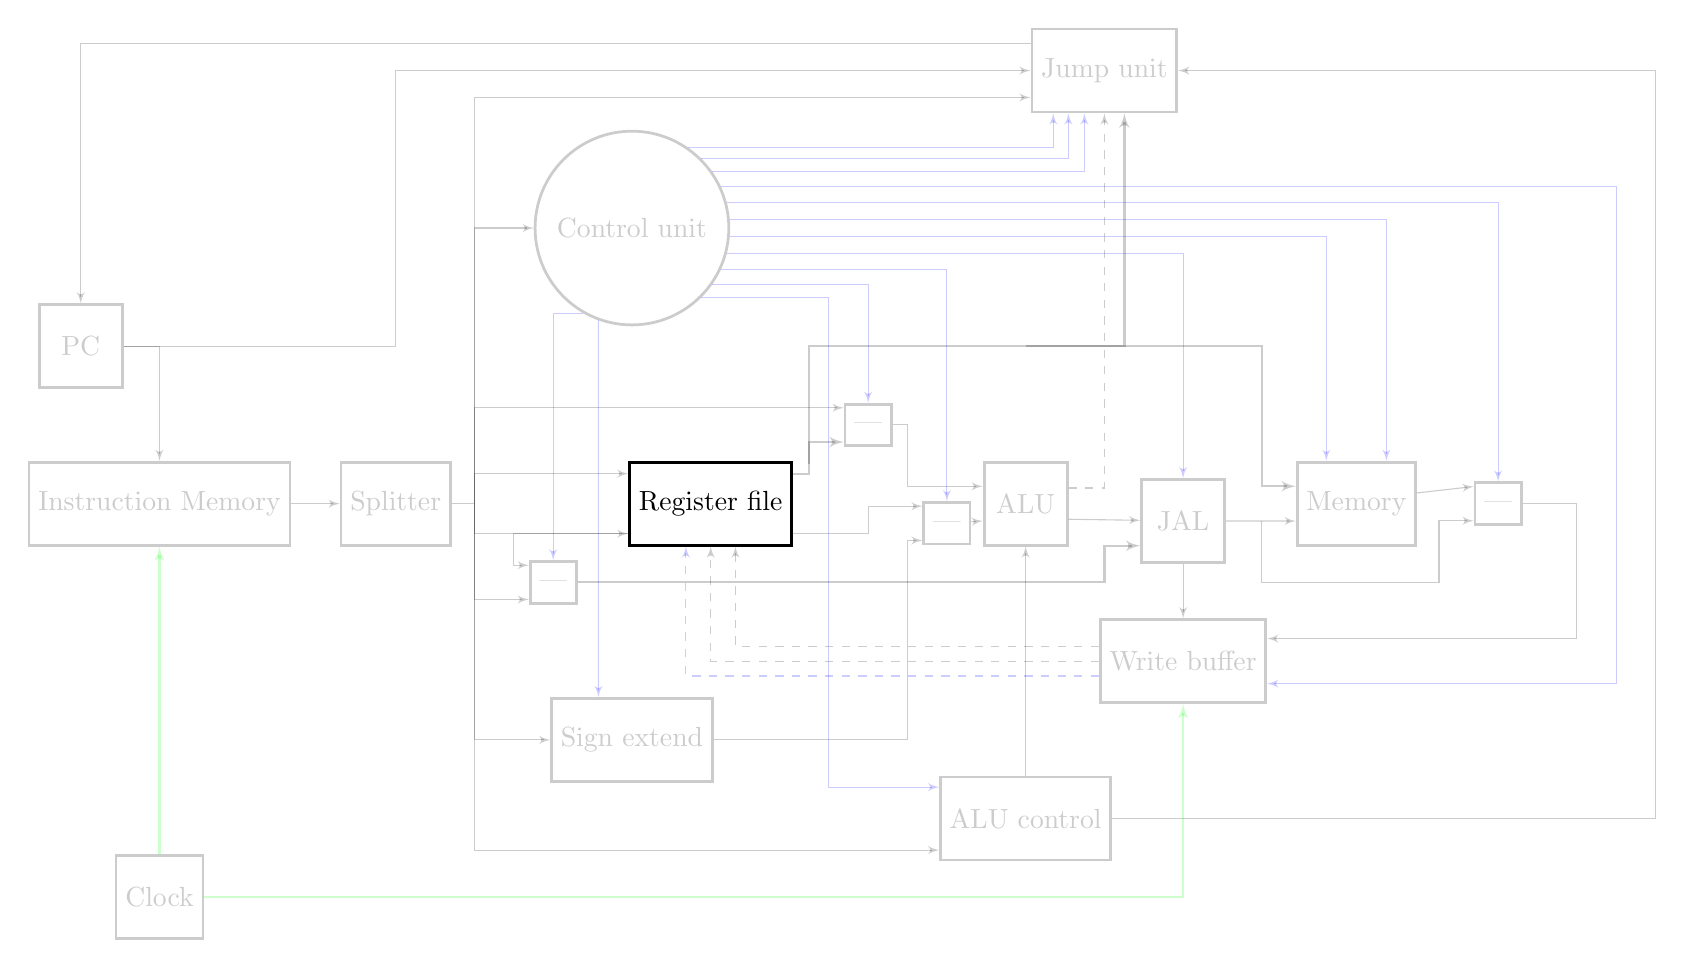
\begin{tikzpicture}
                \node[block] (reg) at (0,0) {Register file};
                \node[opacity=0.2,control] (cont) at (-1,3.5) {Control unit};
                \node[opacity=0.2,block] (jump) at (5,5.5) {Jump unit};
                \node[opacity=0.2,empty] (splitspace) at (-3,0) {};
                \node[opacity=0.2,block] (split) at (-4,0) {Splitter};
                \node[opacity=0.2,block] (if) at (-7,0) {Instruction Memory};
                \node[opacity=0.2,block] (sign) at (-1,-3) {Sign extend};
                \node[opacity=0.2,block] (alu) at (4,0) {ALU};
                \node[opacity=0.2,block] (alucont) at (4,-4) {ALU control};
                \node[opacity=0.2,block] (mem) at (8.2,0) {Memory};
                \node[opacity=0.2,block] (jal) at (6,-0.22) {JAL};
                \node[opacity=0.2,mux] (memread) at (10,0) {|};
                \node[opacity=0.2,mux] (shmt) at (2,1) {|};
                \node[opacity=0.2,mux] (imm) at (3, -0.25) {|};
                \node[opacity=0.2,mux] (regdst) at (-2,-1) {|};
                \node[opacity=0.2,block] (pc) at (-8, 2) {PC};
                \node[opacity=0.2,block] (writebuf) at (6, -2) {Write buffer};

                \path[opacity=0.2,draw, ->] (if) -- (split);
                \path[opacity=0.2,draw, -] (split) -- (splitspace.center);
                \path[opacity=0.2,draw, ->] (splitspace.center) |- (sign);
                \path[opacity=0.2,draw, ->] (splitspace.center) |- (cont);
                \path[opacity=0.2,draw, ->] (splitspace.center) |- (reg.160);
                \path[opacity=0.2,draw, ->] (splitspace.center) |- (reg.200);
                \path[opacity=0.2,draw, ->] (splitspace.center) |- (jump.200);
                \path[opacity=0.2,draw, ->] (splitspace.center) |- (alucont.200);
                \path[opacity=0.2,draw, ->] (splitspace.center) |- (regdst.215);
                \path[opacity=0.2,draw, ->] (splitspace.center) |- (shmt.145);
                \path[opacity=0.2,draw, ->] (reg.200) -| (-2.5, -0.5) |- (regdst.145);
                \path[opacity=0.2,draw, ->] (alucont) -- (alu);
                \path[opacity=0.2,draw, ->] (alucont) -| (12, 0) |- (jump);
                \path[opacity=0.2,draw, ->] (reg.340) -| (2,-0.25) |- (imm.145);
                \path[opacity=0.2,draw, thick, ->] (reg.20) -| (1.25,0.5) |- (shmt.215);
                \path[opacity=0.2,draw, thick, ->] (1.25, 0.5) |- (4, 2) -| (7,1) |- (mem.164);
                \path[opacity=0.2,draw, thick, ->] (4,2) -| (jump.295);
                \path[opacity=0.2,draw, ->] (shmt) -| (2.5, 0.5) |- (alu.158);
                \path[opacity=0.2,draw, dashed, ->] (alu.20) -| (jump);
                \path[opacity=0.2,draw, ->] (alu.340) -- (jal);
                \path[opacity=0.2,draw, ->] (jal) -- (mem.196);
                \path[opacity=0.2,draw, ->] (imm) -- (alu.202);
                \path[opacity=0.2,draw, ->] (7, -0.22) |- (8, -1) -| (9.25,-0.5) |- (memread.215);
                \path[opacity=0.2,draw, ->] (mem.10) -- (memread.145);
                \path[opacity=0.2,draw, ->] (sign) -| (2.5, -1) |- (imm.215);
                \path[opacity=0.2,draw, thick, ->] (regdst) -| (5, -0.6) |- (jal.210);
                \path[opacity=0.2,draw, ->] (pc) -| (if);
                \path[opacity=0.2,draw, ->] (pc) -| (-4, 4) |- (jump);
                \path[opacity=0.2,draw, ->] (jump.160) -| (pc);
                \path[opacity=0.2,draw, ->] (jal) -- (writebuf);
                \path[opacity=0.2,draw, ->] (memread) -| (11, -1) |- (writebuf.15);
                \path[opacity=0.2,draw, dashed, ->] (writebuf.170) -| (reg.300);
                \path[opacity=0.2,draw, dashed, ->] (writebuf) -| (reg);
                \path[opacity=0.2,draw, dashed, ->, color=blue] (writebuf.190) -| (reg.240);

                \path[opacity=0.2,draw, ->, color=blue] (cont.55) -| (jump.220);
                \path[opacity=0.2,draw, ->, color=blue] (cont.45) -| (jump.230);
                \path[opacity=0.2,draw, ->, color=blue] (cont.35) -| (jump.245);
                \path[opacity=0.2,draw, ->, color=blue] (cont.25) -| (11.5,0) |-(writebuf.345);
                \path[opacity=0.2,draw, ->, color=blue] (cont.15) -| (memread);
                \path[opacity=0.2,draw, ->, color=blue] (cont.5) -| (mem.55);
                \path[opacity=0.2,draw, ->, color=blue] (cont.355) -| (mem.125);
                \path[opacity=0.2,draw, ->, color=blue] (cont.345) -| (jal);
                \path[opacity=0.2,draw, ->, color=blue] (cont.335) -| (imm);
                \path[opacity=0.2,draw, ->, color=blue] (cont.325) -| (shmt);
                \path[opacity=0.2,draw, ->, color=blue] (cont.315) -| (1.5, 0.5) |- (alucont.160);
                %\path[opacity=0.2,draw, ->, color=blue] (cont.305) -- (reg.110);
                \path[opacity=0.2,draw, ->, color=blue] (cont.250) -- (sign.128);
                \path[opacity=0.2,draw, ->, color=blue] (cont.240) -| (regdst);

                \node[opacity=0.2,block] (clock) at (-7, -5) {Clock};
                \path[opacity=0.2,draw, ->, thick, color=green] (clock) -- (if);
                \path[opacity=0.2,draw, ->, thick, color=green] (clock) -| (writebuf);
            \end{tikzpicture}
        }
    \end{figure}
\end{frame}
\subsection{Background}
\begin{frame}
    The register file is the component that holds values for the processor. It
    is the first step in a memory hierarchy, and is thus the fastest memory
    available.

    \vspace{\baselineskip}
    There are 32 registers in a 32-bit MIPS processor, each holding a 32-bit
    value. The registers are divided into groups based on their usage. This
    does not matter from a hardware perspective, except for register 0, which
    is immutable and always 0.
\end{frame}
\begin{frame}
    The register file has 5 inputs:
    \begin{itemize}
        \item Read address A
        \item Read address B
        \item Write enabled
        \item Write address
        \item Write data
    \end{itemize}
    And it has 2 outputs:
    \begin{itemize}
        \item Output A
        \item Output B
    \end{itemize}
\end{frame}
\begin{frame}
    \begin{figure}
        \centering
        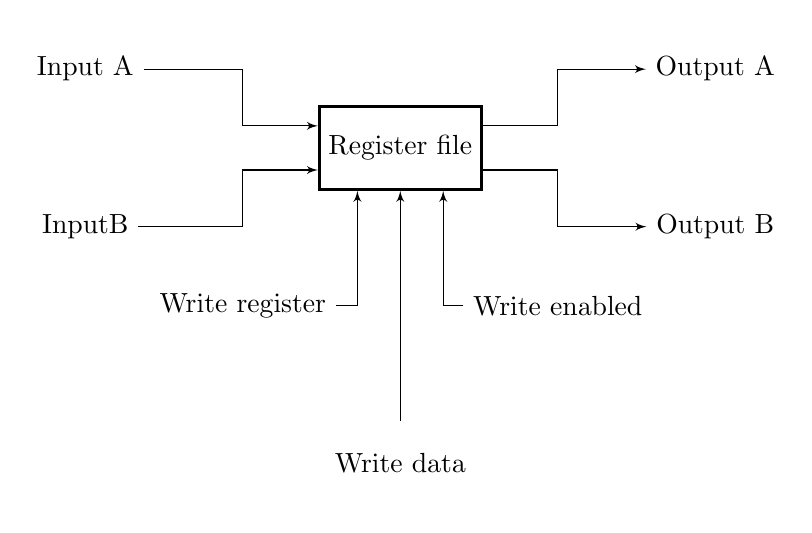
\begin{tikzpicture}[node distance=2cm]
            \node[empty] (inputa) {Input A};
            \node[empty, below of=inputa] (inputb) {InputB};

            \node[empty, right of=inputa] (spacing) at ($(inputa)!0.5!(inputb)$) {};
            \node[block, right of=spacing] (register) {Register file};
            \node[empty, below of=register] (wdspace) {};
            \node[empty, below of=wdspace] (writedata) {Write data};
            \node[empty, left of=wdspace] (write) {Write register};
            \node[empty, right of=wdspace] (writeenabled) {Write enabled};

            \node[empty, right of=inputa] (space) {};
            \node[empty, right of=space] (spacee) {};
            \node[empty, right of=spacee] (spaceee) {};
            \node[empty, right of=spaceee] (outputa) {Output A};
            \node[empty, below of=outputa] (outputb) {Output B};
            \node[empty, left of=outputb] (bspace) {};

            \path[draw, -] (inputa) -| (spacing.north);
            \path[draw, ->] (spacing.north) |- (register.165);
            \path[draw, -] (inputb) -| (spacing.south);
            \path[draw, ->] (spacing.south) |- (register.195);

            \path[draw, ->] (write) -| (register.225);
            \path[draw, ->] (writedata) -- (register);
            \path[draw, ->] (writeenabled) -| (register.315);

            \path[draw, -] (register.345) -| (bspace.north);
            \path[draw, ->] (bspace.north) |- (outputb);
            \path[draw, -] (register.15) -| (spaceee.south);
            \path[draw, ->] (spaceee.south) |- (outputa);
        \end{tikzpicture}
        \label{fig:register}
    \end{figure}
\end{frame}
\begin{frame}
    It is important to ensure that when an instruction reads from the register
    file, it should always get the latest data. I.e. if a instruction reads
    from the same register as the previous instruction wrote to, it should read
    the value written by the previous instruction.

    \vspace{\baselineskip}
    This is easy to fix in the single cycle processor, as we just need to write
    before reading.
\end{frame}
\subsection{Implementation}
\begin{frame}
    To implement the register file in SME, we construct a process holding an
    int array. It should have the inputs and outputs as specified.

    \vspace{\baselineskip}
    Upon receiving input, it should write the write data into the array at the
    given write address, if the \texttt{RegWrite} flag has been set. Then it
    should output the value at read address A on output A, and the analogous
    for read address B and output B.

    \vspace{\baselineskip}
    Note: remember that register 0 is immutable and always 0.
\end{frame}
\subsection{Testing}
\begin{frame}
    Testing the register file is very trivial. We construct a tester process,
    which sends some values on the write data bus, along with some addresses
    and the \texttt{RegWrite} flag set.

    \vspace{\baselineskip}
    Then it just sends some addresses on the Read address A and Read address B
    buses, and verifies that the register file outputs the values stored at
    these addresses.

    \vspace{\baselineskip}
    It is also important to verify that the behaviour of register zero is as it
    should be.
\end{frame}

\section{ALU}
\begin{frame}
    \begin{figure}
        \centering
        \scalebox{0.5}{
            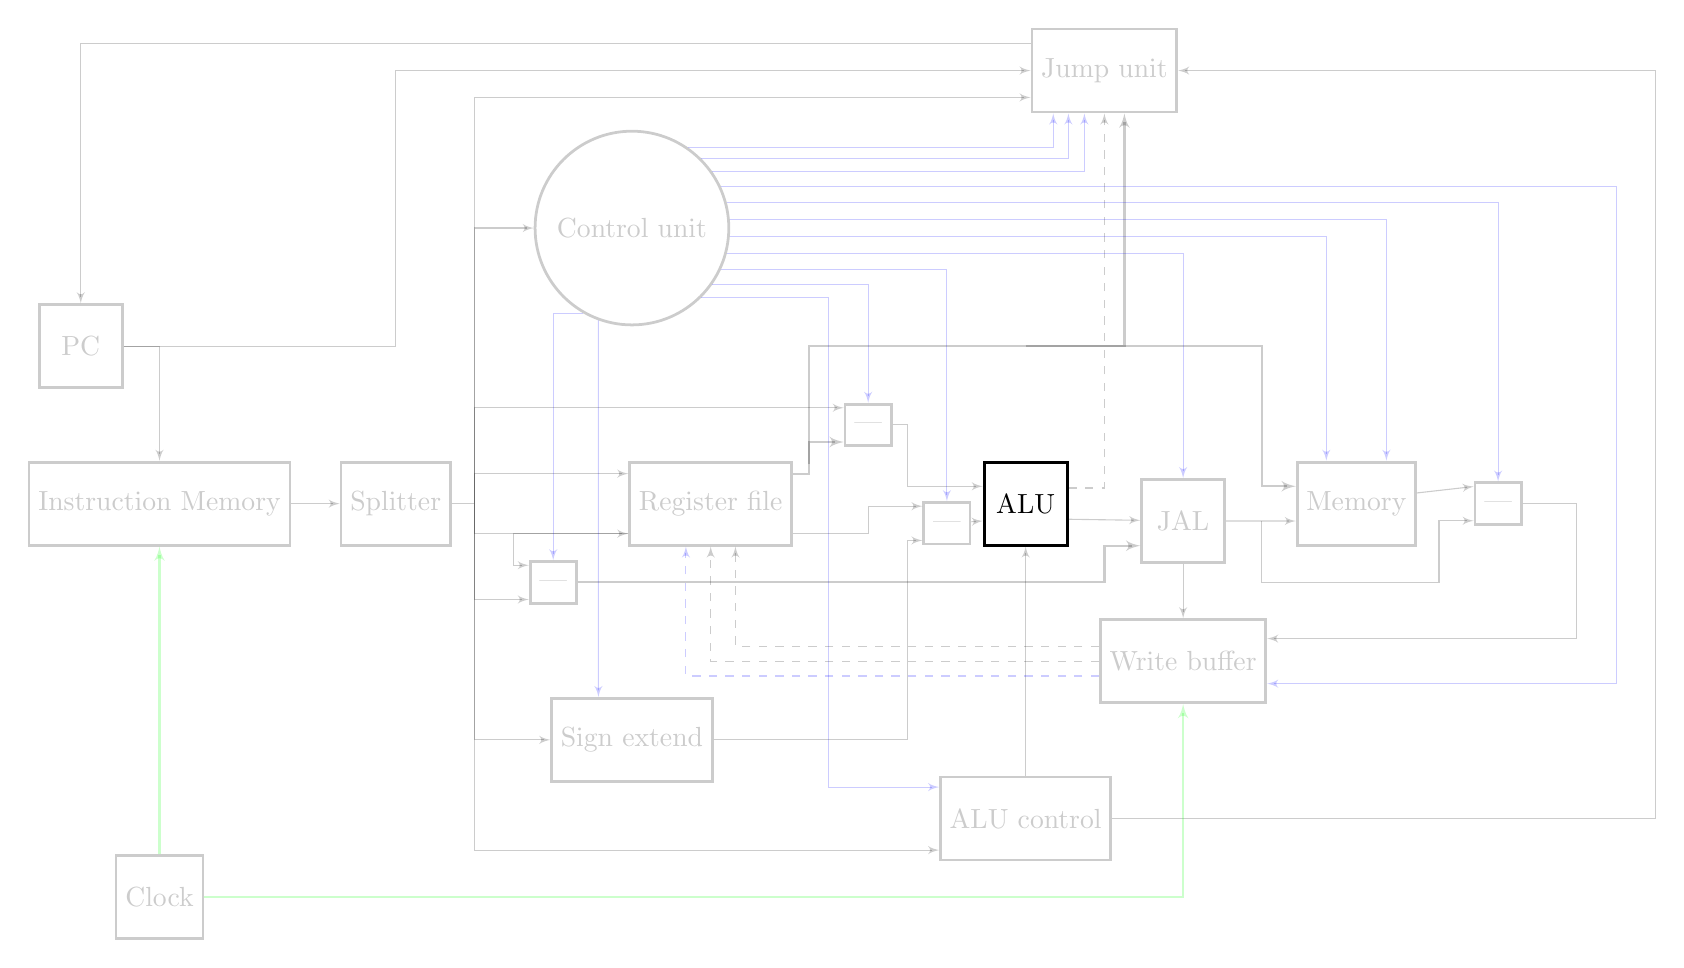
\begin{tikzpicture}
                \node[opacity=0.2,block] (reg) at (0,0) {Register file};
                \node[opacity=0.2,control] (cont) at (-1,3.5) {Control unit};
                \node[opacity=0.2,block] (jump) at (5,5.5) {Jump unit};
                \node[opacity=0.2,empty] (splitspace) at (-3,0) {};
                \node[opacity=0.2,block] (split) at (-4,0) {Splitter};
                \node[opacity=0.2,block] (if) at (-7,0) {Instruction Memory};
                \node[opacity=0.2,block] (sign) at (-1,-3) {Sign extend};
                \node[block] (alu) at (4,0) {ALU};
                \node[opacity=0.2,block] (alucont) at (4,-4) {ALU control};
                \node[opacity=0.2,block] (mem) at (8.2,0) {Memory};
                \node[opacity=0.2,block] (jal) at (6,-0.22) {JAL};
                \node[opacity=0.2,mux] (memread) at (10,0) {|};
                \node[opacity=0.2,mux] (shmt) at (2,1) {|};
                \node[opacity=0.2,mux] (imm) at (3, -0.25) {|};
                \node[opacity=0.2,mux] (regdst) at (-2,-1) {|};
                \node[opacity=0.2,block] (pc) at (-8, 2) {PC};
                \node[opacity=0.2,block] (writebuf) at (6, -2) {Write buffer};

                \path[opacity=0.2,draw, ->] (if) -- (split);
                \path[opacity=0.2,draw, -] (split) -- (splitspace.center);
                \path[opacity=0.2,draw, ->] (splitspace.center) |- (sign);
                \path[opacity=0.2,draw, ->] (splitspace.center) |- (cont);
                \path[opacity=0.2,draw, ->] (splitspace.center) |- (reg.160);
                \path[opacity=0.2,draw, ->] (splitspace.center) |- (reg.200);
                \path[opacity=0.2,draw, ->] (splitspace.center) |- (jump.200);
                \path[opacity=0.2,draw, ->] (splitspace.center) |- (alucont.200);
                \path[opacity=0.2,draw, ->] (splitspace.center) |- (regdst.215);
                \path[opacity=0.2,draw, ->] (splitspace.center) |- (shmt.145);
                \path[opacity=0.2,draw, ->] (reg.200) -| (-2.5, -0.5) |- (regdst.145);
                \path[opacity=0.2,draw, ->] (alucont) -- (alu);
                \path[opacity=0.2,draw, ->] (alucont) -| (12, 0) |- (jump);
                \path[opacity=0.2,draw, ->] (reg.340) -| (2,-0.25) |- (imm.145);
                \path[opacity=0.2,draw, thick, ->] (reg.20) -| (1.25,0.5) |- (shmt.215);
                \path[opacity=0.2,draw, thick, ->] (1.25, 0.5) |- (4, 2) -| (7,1) |- (mem.164);
                \path[opacity=0.2,draw, thick, ->] (4,2) -| (jump.295);
                \path[opacity=0.2,draw, ->] (shmt) -| (2.5, 0.5) |- (alu.158);
                \path[opacity=0.2,draw, dashed, ->] (alu.20) -| (jump);
                \path[opacity=0.2,draw, ->] (alu.340) -- (jal);
                \path[opacity=0.2,draw, ->] (jal) -- (mem.196);
                \path[opacity=0.2,draw, ->] (imm) -- (alu.202);
                \path[opacity=0.2,draw, ->] (7, -0.22) |- (8, -1) -| (9.25,-0.5) |- (memread.215);
                \path[opacity=0.2,draw, ->] (mem.10) -- (memread.145);
                \path[opacity=0.2,draw, ->] (sign) -| (2.5, -1) |- (imm.215);
                \path[opacity=0.2,draw, thick, ->] (regdst) -| (5, -0.6) |- (jal.210);
                \path[opacity=0.2,draw, ->] (pc) -| (if);
                \path[opacity=0.2,draw, ->] (pc) -| (-4, 4) |- (jump);
                \path[opacity=0.2,draw, ->] (jump.160) -| (pc);
                \path[opacity=0.2,draw, ->] (jal) -- (writebuf);
                \path[opacity=0.2,draw, ->] (memread) -| (11, -1) |- (writebuf.15);
                \path[opacity=0.2,draw, dashed, ->] (writebuf.170) -| (reg.300);
                \path[opacity=0.2,draw, dashed, ->] (writebuf) -| (reg);
                \path[opacity=0.2,draw, dashed, ->, color=blue] (writebuf.190) -| (reg.240);

                \path[opacity=0.2,draw, ->, color=blue] (cont.55) -| (jump.220);
                \path[opacity=0.2,draw, ->, color=blue] (cont.45) -| (jump.230);
                \path[opacity=0.2,draw, ->, color=blue] (cont.35) -| (jump.245);
                \path[opacity=0.2,draw, ->, color=blue] (cont.25) -| (11.5,0) |-(writebuf.345);
                \path[opacity=0.2,draw, ->, color=blue] (cont.15) -| (memread);
                \path[opacity=0.2,draw, ->, color=blue] (cont.5) -| (mem.55);
                \path[opacity=0.2,draw, ->, color=blue] (cont.355) -| (mem.125);
                \path[opacity=0.2,draw, ->, color=blue] (cont.345) -| (jal);
                \path[opacity=0.2,draw, ->, color=blue] (cont.335) -| (imm);
                \path[opacity=0.2,draw, ->, color=blue] (cont.325) -| (shmt);
                \path[opacity=0.2,draw, ->, color=blue] (cont.315) -| (1.5, 0.5) |- (alucont.160);
                %\path[opacity=0.2,draw, ->, color=blue] (cont.305) -- (reg.110);
                \path[opacity=0.2,draw, ->, color=blue] (cont.250) -- (sign.128);
                \path[opacity=0.2,draw, ->, color=blue] (cont.240) -| (regdst);

                \node[opacity=0.2,block] (clock) at (-7, -5) {Clock};
                \path[opacity=0.2,draw, ->, thick, color=green] (clock) -- (if);
                \path[opacity=0.2,draw, ->, thick, color=green] (clock) -| (writebuf);
            \end{tikzpicture}
        }
    \end{figure}
\end{frame}
\subsection{Background}
\begin{frame}
    The ALU (Arithmetic Logic Unit) is the part of the processor, which makes
    the actual computation.

    \vspace{\baselineskip}
    It has three inputs:
    \begin{itemize}
        \item Input A
        \item Input B
        \item ALU opcode
    \end{itemize}
    and produces two outputs:
    \begin{itemize}
        \item Result
        \item Zero flag
    \end{itemize}
\end{frame}
\begin{frame}
    \begin{figure}
        \centering
        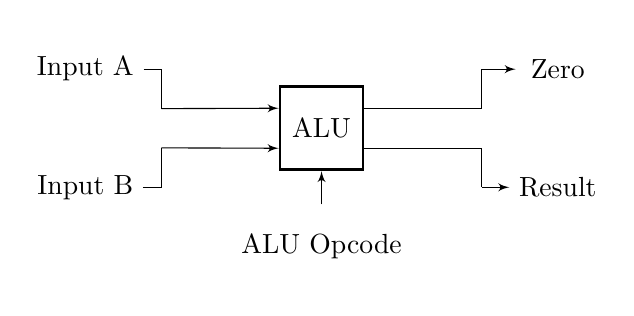
\begin{tikzpicture} [node distance=1.5cm]
            \node[empty] (ina) {Input A};
            \node[empty, below of=ina] (inb) {Input B};
            \node[empty, right of=inputa] (spacing) at ($(ina)!0.5!(inb)$) {};
            \node[block, right of=spacing] (alu) {ALU};
            \node[empty, right of=ina] (align0) {};
            \node[empty, right of=align0] (align1) {};
            \node[empty, right of=align1] (align2) {};
            \node[empty, right of=align2] (result) {Zero};
            \node[empty, below of=result] (zero) {Result};
            \node[empty, left of=zero] (align3) {};
            \node[empty, below of=alu] (aluop) {ALU Opcode};

            \path[draw, -] (ina.east) -| (spacing.155);
            \path[draw, ->] (spacing.155) -- (alu.155);
            \path[draw, -] (inb.east) -| (spacing.205);
            \path[draw, ->] (spacing.205) -- (alu.205);
            \path[draw, ->] (aluop) -- (alu);
            \path[draw, -] (alu.25) -| (align2.east);
            \path[draw, ->] (align2.east) -- (result);
            \path[draw, -] (alu.335) -| (align3.east);
            \path[draw, ->] (align3.east) -- (zero);
        \end{tikzpicture}
        \label{fig:alu}
    \end{figure}
\end{frame}
\begin{frame}
    Upon receiving all of its inputs, it takes the values from Input A and
    Input B, performs the operation specified by the ALU opcode on them,
    outputs the result on the Result bus, and finally sets the Zero flag to
    \texttt{1}, if the result was 0.
\end{frame}
\subsection{Implementation}
\begin{frame}
    As with the register file, to implement the ALU, we construct a process in
    SME. It should have the inputs and outputs as specified.

    \vspace{\baselineskip}
    The process should start by reading the values from Input A and Input B.
    Then, it should \texttt{switch} on the value from the ALU opcode, and based
    on that perform the associated operation. Finally it should output on the
    Zero flag, if the result of the computation was 0.

    \vspace{\baselineskip}
    Note: the \texttt{switch} on the ALU opcode can become more human readable
    by using an \texttt{enum}
\end{frame}
\begin{frame}
    We follow the procedure in the book, and make sure the ALU support the
    following operations:
    \begin{itemize}
        \item \texttt{add}
        \item \texttt{sub}
        \item \texttt{and}
        \item \texttt{or}
        \item \texttt{slt}
    \end{itemize}
    We will be adding more operations later on.
\end{frame}
\subsection{Testing}
\begin{frame}
    Testing the ALU is like the Register File, very trivial. Construct a tester
    process, which:
    \begin{itemize}
        \item Sends values on the Input A, Input B and ALU Opcode busses
        \item Reads the values from the Result and Zero Busses
        \item Verifies that the read values are as expected
    \end{itemize}
\end{frame}

\section{Control Unit}
\begin{frame}
    \begin{figure}
        \centering
        \scalebox{0.5}{
            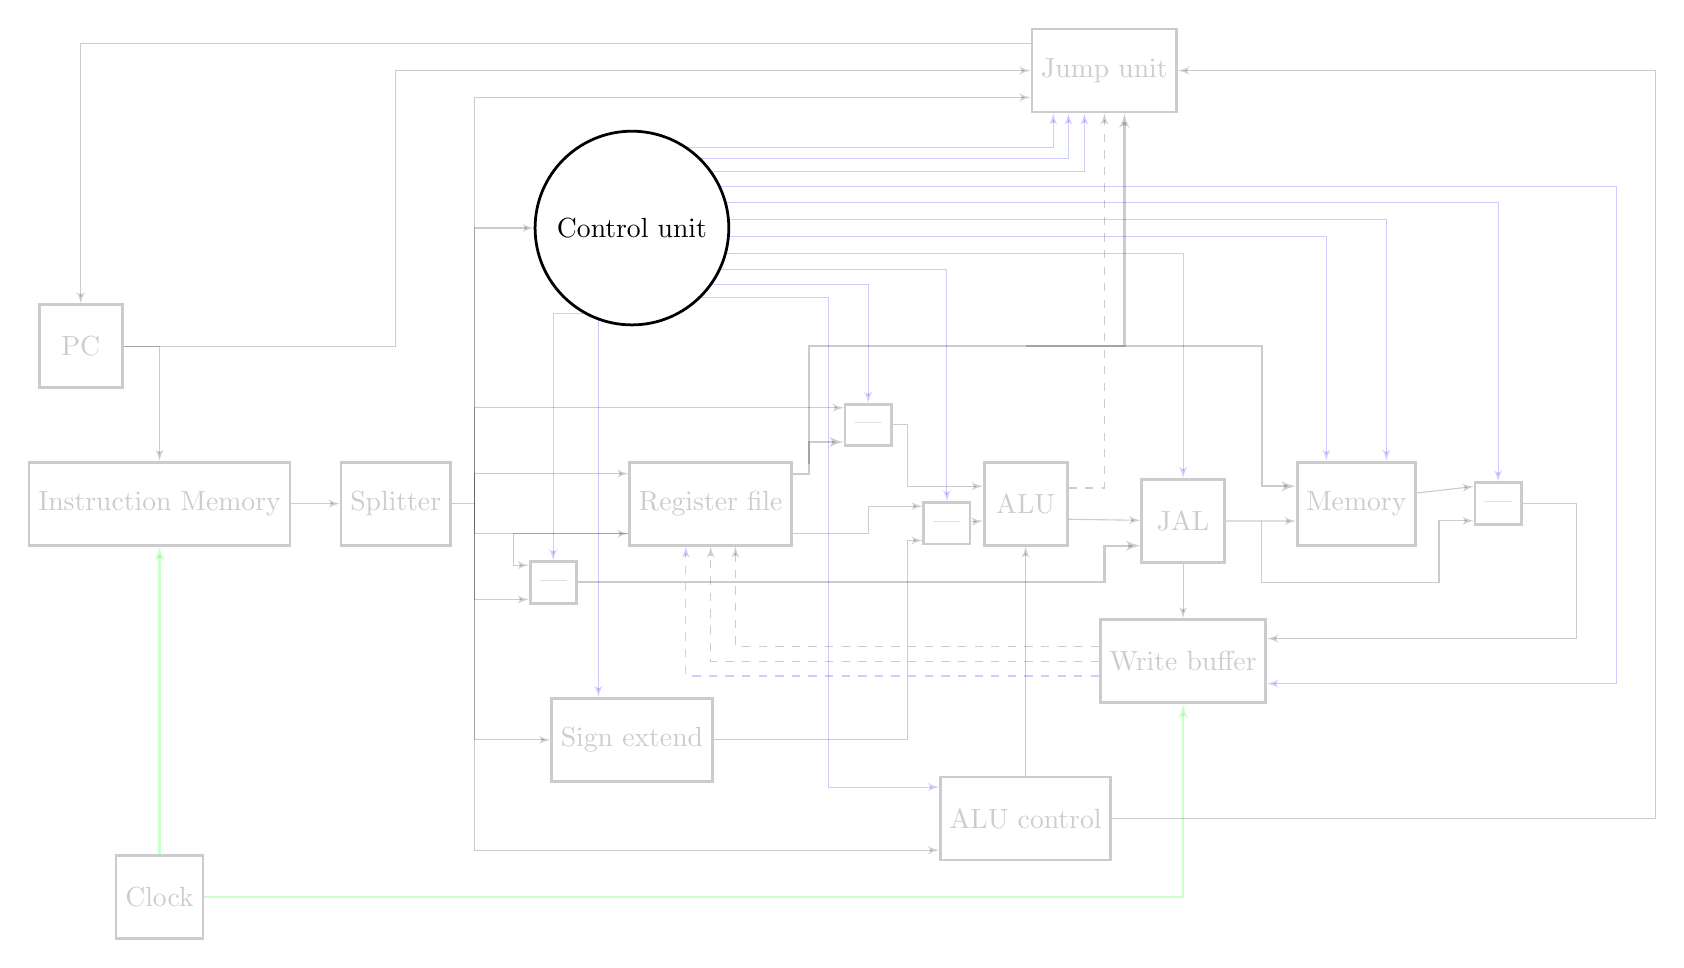
\begin{tikzpicture}
                \node[opacity=0.2,block] (reg) at (0,0) {Register file};
                \node[control] (cont) at (-1,3.5) {Control unit};
                \node[opacity=0.2,block] (jump) at (5,5.5) {Jump unit};
                \node[opacity=0.2,empty] (splitspace) at (-3,0) {};
                \node[opacity=0.2,block] (split) at (-4,0) {Splitter};
                \node[opacity=0.2,block] (if) at (-7,0) {Instruction Memory};
                \node[opacity=0.2,block] (sign) at (-1,-3) {Sign extend};
                \node[opacity=0.2,block] (alu) at (4,0) {ALU};
                \node[opacity=0.2,block] (alucont) at (4,-4) {ALU control};
                \node[opacity=0.2,block] (mem) at (8.2,0) {Memory};
                \node[opacity=0.2,block] (jal) at (6,-0.22) {JAL};
                \node[opacity=0.2,mux] (memread) at (10,0) {|};
                \node[opacity=0.2,mux] (shmt) at (2,1) {|};
                \node[opacity=0.2,mux] (imm) at (3, -0.25) {|};
                \node[opacity=0.2,mux] (regdst) at (-2,-1) {|};
                \node[opacity=0.2,block] (pc) at (-8, 2) {PC};
                \node[opacity=0.2,block] (writebuf) at (6, -2) {Write buffer};

                \path[opacity=0.2,draw, ->] (if) -- (split);
                \path[opacity=0.2,draw, -] (split) -- (splitspace.center);
                \path[opacity=0.2,draw, ->] (splitspace.center) |- (sign);
                \path[opacity=0.2,draw, ->] (splitspace.center) |- (cont);
                \path[opacity=0.2,draw, ->] (splitspace.center) |- (reg.160);
                \path[opacity=0.2,draw, ->] (splitspace.center) |- (reg.200);
                \path[opacity=0.2,draw, ->] (splitspace.center) |- (jump.200);
                \path[opacity=0.2,draw, ->] (splitspace.center) |- (alucont.200);
                \path[opacity=0.2,draw, ->] (splitspace.center) |- (regdst.215);
                \path[opacity=0.2,draw, ->] (splitspace.center) |- (shmt.145);
                \path[opacity=0.2,draw, ->] (reg.200) -| (-2.5, -0.5) |- (regdst.145);
                \path[opacity=0.2,draw, ->] (alucont) -- (alu);
                \path[opacity=0.2,draw, ->] (alucont) -| (12, 0) |- (jump);
                \path[opacity=0.2,draw, ->] (reg.340) -| (2,-0.25) |- (imm.145);
                \path[opacity=0.2,draw, thick, ->] (reg.20) -| (1.25,0.5) |- (shmt.215);
                \path[opacity=0.2,draw, thick, ->] (1.25, 0.5) |- (4, 2) -| (7,1) |- (mem.164);
                \path[opacity=0.2,draw, thick, ->] (4,2) -| (jump.295);
                \path[opacity=0.2,draw, ->] (shmt) -| (2.5, 0.5) |- (alu.158);
                \path[opacity=0.2,draw, dashed, ->] (alu.20) -| (jump);
                \path[opacity=0.2,draw, ->] (alu.340) -- (jal);
                \path[opacity=0.2,draw, ->] (jal) -- (mem.196);
                \path[opacity=0.2,draw, ->] (imm) -- (alu.202);
                \path[opacity=0.2,draw, ->] (7, -0.22) |- (8, -1) -| (9.25,-0.5) |- (memread.215);
                \path[opacity=0.2,draw, ->] (mem.10) -- (memread.145);
                \path[opacity=0.2,draw, ->] (sign) -| (2.5, -1) |- (imm.215);
                \path[opacity=0.2,draw, thick, ->] (regdst) -| (5, -0.6) |- (jal.210);
                \path[opacity=0.2,draw, ->] (pc) -| (if);
                \path[opacity=0.2,draw, ->] (pc) -| (-4, 4) |- (jump);
                \path[opacity=0.2,draw, ->] (jump.160) -| (pc);
                \path[opacity=0.2,draw, ->] (jal) -- (writebuf);
                \path[opacity=0.2,draw, ->] (memread) -| (11, -1) |- (writebuf.15);
                \path[opacity=0.2,draw, dashed, ->] (writebuf.170) -| (reg.300);
                \path[opacity=0.2,draw, dashed, ->] (writebuf) -| (reg);
                \path[opacity=0.2,draw, dashed, ->, color=blue] (writebuf.190) -| (reg.240);

                \path[opacity=0.2,draw, ->, color=blue] (cont.55) -| (jump.220);
                \path[opacity=0.2,draw, ->, color=blue] (cont.45) -| (jump.230);
                \path[opacity=0.2,draw, ->, color=blue] (cont.35) -| (jump.245);
                \path[opacity=0.2,draw, ->, color=blue] (cont.25) -| (11.5,0) |-(writebuf.345);
                \path[opacity=0.2,draw, ->, color=blue] (cont.15) -| (memread);
                \path[opacity=0.2,draw, ->, color=blue] (cont.5) -| (mem.55);
                \path[opacity=0.2,draw, ->, color=blue] (cont.355) -| (mem.125);
                \path[opacity=0.2,draw, ->, color=blue] (cont.345) -| (jal);
                \path[opacity=0.2,draw, ->, color=blue] (cont.335) -| (imm);
                \path[opacity=0.2,draw, ->, color=blue] (cont.325) -| (shmt);
                \path[opacity=0.2,draw, ->, color=blue] (cont.315) -| (1.5, 0.5) |- (alucont.160);
                %\path[opacity=0.2,draw, ->, color=blue] (cont.305) -- (reg.110);
                \path[opacity=0.2,draw, ->, color=blue] (cont.250) -- (sign.128);
                \path[opacity=0.2,draw, ->, color=blue] (cont.240) -| (regdst);

                \node[opacity=0.2,block] (clock) at (-7, -5) {Clock};
                \path[opacity=0.2,draw, ->, thick, color=green] (clock) -- (if);
                \path[opacity=0.2,draw, ->, thick, color=green] (clock) -| (writebuf);
            \end{tikzpicture}
        }
    \end{figure}
\end{frame}
\subsection{Background}
\begin{frame}
    The Control Unit is part of the decoding step. It takes the opcode of the
    instruction, and based on the opcode, it sets control flags, which are used
    troughout the processor.

    Since we are following the book, we start by having the following flags:
    \begin{itemize}
        \item \texttt{RegDst}
        \item \texttt{Branch}
        \item \texttt{MemRead}
        \item \texttt{MemToReg}
        \item \texttt{ALUOp}
        \item \texttt{MemWrite}
        \item \texttt{ALUSrc}
        \item \texttt{RegWrite}
    \end{itemize}
\end{frame}
\begin{frame}
    \begin{figure}
        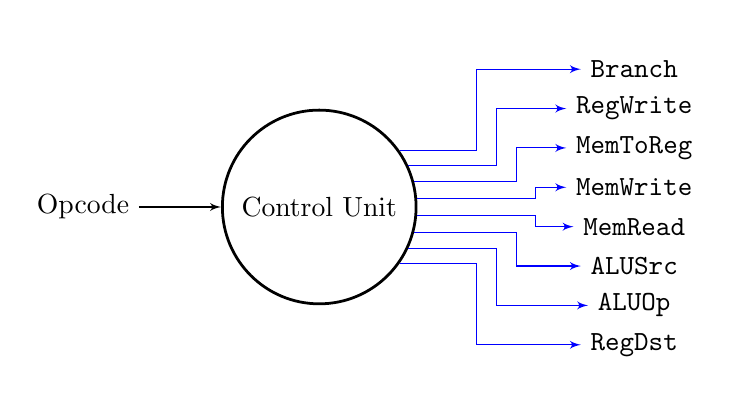
\begin{tikzpicture}
            \node[control] (cont)   at (0,  0)   {Control Unit};
            \node[empty] (opcode)   at (-3, 0)   {Opcode};
            \node[empty] (branch)   at (4,  1.75) {\texttt{Branch}};
            \node[empty] (regwrite) at (4,  1.25) {\texttt{RegWrite}};
            \node[empty] (memtoreg) at (4,  0.75) {\texttt{MemToReg}};
            \node[empty] (memwrite) at (4,  0.25) {\texttt{MemWrite}};
            \node[empty] (memread)  at (4, -0.25) {\texttt{MemRead}};
            \node[empty] (alusrc)   at (4, -0.75) {\texttt{ALUSrc}};
            \node[empty] (aluop)    at (4, -1.25) {\texttt{ALUOp}};
            \node[empty] (regdst)   at (4, -1.75) {\texttt{RegDst}};

            \path[draw, ->] (opcode) -- (cont);

            \path[draw, ->, color=blue] (cont.35)  -| (2,1.5) |- (branch);
            \path[draw, ->, color=blue] (cont.25)  -| (2.25,1) |- (regwrite);
            \path[draw, ->, color=blue] (cont.15)  -| (2.5,0.5) |- (memtoreg);
            \path[draw, ->, color=blue] (cont.5)   -| (2.75,0.125) |- (memwrite);
            \path[draw, ->, color=blue] (cont.355) -| (2.75,-0.125) |- (memread);
            \path[draw, ->, color=blue] (cont.345) -| (2.5,-0.5) |- (alusrc);
            \path[draw, ->, color=blue] (cont.335) -| (2.25,-1) |- (aluop);
            \path[draw, ->, color=blue] (cont.325) -| (2,-1.5) |- (regdst);
        \end{tikzpicture}
    \end{figure}
\end{frame}
\subsection{Implementation \& Testing}
\begin{frame}
    The book describes the needed logic, but it is not very extensible. To
    solve this, we construct our own Control Unit. The process should have a
    \texttt{switch} statement on the opcode. For each case, we set the flags
    accordingly.

    \vspace{\baselineskip}
    Note: as with the ALU, the source code becomes more readably with a
    \texttt{enum} on the opcode and on the ALUOp.

    \vspace{\baselineskip}
    As before, we construct a tester process, which sends different opcodes to
    the Control Unit, and verifies its output. It should be tested whether or
    not all of the expected input opcodes performs as expected.
\end{frame}
\section{ALU Control}
\begin{frame}
    \begin{figure}
        \centering
        \scalebox{0.5}{
            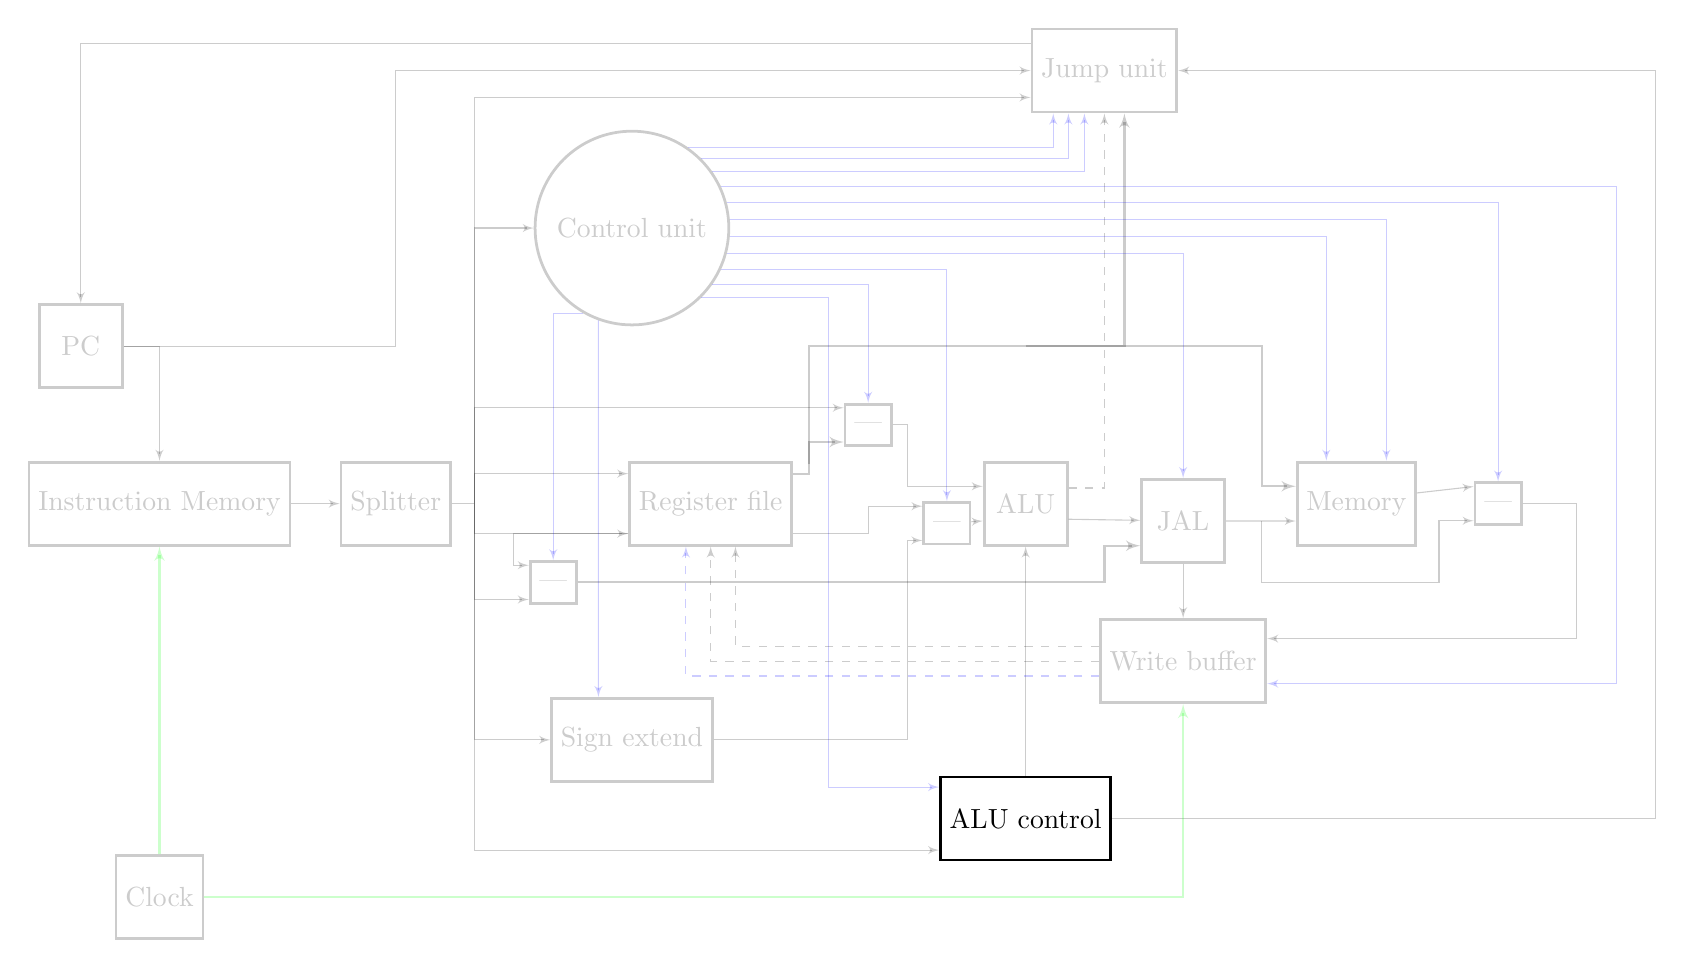
\begin{tikzpicture}
                \node[opacity=0.2,block] (reg) at (0,0) {Register file};
                \node[opacity=0.2,control] (cont) at (-1,3.5) {Control unit};
                \node[opacity=0.2,block] (jump) at (5,5.5) {Jump unit};
                \node[opacity=0.2,empty] (splitspace) at (-3,0) {};
                \node[opacity=0.2,block] (split) at (-4,0) {Splitter};
                \node[opacity=0.2,block] (if) at (-7,0) {Instruction Memory};
                \node[opacity=0.2,block] (sign) at (-1,-3) {Sign extend};
                \node[opacity=0.2,block] (alu) at (4,0) {ALU};
                \node[block] (alucont) at (4,-4) {ALU control};
                \node[opacity=0.2,block] (mem) at (8.2,0) {Memory};
                \node[opacity=0.2,block] (jal) at (6,-0.22) {JAL};
                \node[opacity=0.2,mux] (memread) at (10,0) {|};
                \node[opacity=0.2,mux] (shmt) at (2,1) {|};
                \node[opacity=0.2,mux] (imm) at (3, -0.25) {|};
                \node[opacity=0.2,mux] (regdst) at (-2,-1) {|};
                \node[opacity=0.2,block] (pc) at (-8, 2) {PC};
                \node[opacity=0.2,block] (writebuf) at (6, -2) {Write buffer};

                \path[opacity=0.2,draw, ->] (if) -- (split);
                \path[opacity=0.2,draw, -] (split) -- (splitspace.center);
                \path[opacity=0.2,draw, ->] (splitspace.center) |- (sign);
                \path[opacity=0.2,draw, ->] (splitspace.center) |- (cont);
                \path[opacity=0.2,draw, ->] (splitspace.center) |- (reg.160);
                \path[opacity=0.2,draw, ->] (splitspace.center) |- (reg.200);
                \path[opacity=0.2,draw, ->] (splitspace.center) |- (jump.200);
                \path[opacity=0.2,draw, ->] (splitspace.center) |- (alucont.200);
                \path[opacity=0.2,draw, ->] (splitspace.center) |- (regdst.215);
                \path[opacity=0.2,draw, ->] (splitspace.center) |- (shmt.145);
                \path[opacity=0.2,draw, ->] (reg.200) -| (-2.5, -0.5) |- (regdst.145);
                \path[opacity=0.2,draw, ->] (alucont) -- (alu);
                \path[opacity=0.2,draw, ->] (alucont) -| (12, 0) |- (jump);
                \path[opacity=0.2,draw, ->] (reg.340) -| (2,-0.25) |- (imm.145);
                \path[opacity=0.2,draw, thick, ->] (reg.20) -| (1.25,0.5) |- (shmt.215);
                \path[opacity=0.2,draw, thick, ->] (1.25, 0.5) |- (4, 2) -| (7,1) |- (mem.164);
                \path[opacity=0.2,draw, thick, ->] (4,2) -| (jump.295);
                \path[opacity=0.2,draw, ->] (shmt) -| (2.5, 0.5) |- (alu.158);
                \path[opacity=0.2,draw, dashed, ->] (alu.20) -| (jump);
                \path[opacity=0.2,draw, ->] (alu.340) -- (jal);
                \path[opacity=0.2,draw, ->] (jal) -- (mem.196);
                \path[opacity=0.2,draw, ->] (imm) -- (alu.202);
                \path[opacity=0.2,draw, ->] (7, -0.22) |- (8, -1) -| (9.25,-0.5) |- (memread.215);
                \path[opacity=0.2,draw, ->] (mem.10) -- (memread.145);
                \path[opacity=0.2,draw, ->] (sign) -| (2.5, -1) |- (imm.215);
                \path[opacity=0.2,draw, thick, ->] (regdst) -| (5, -0.6) |- (jal.210);
                \path[opacity=0.2,draw, ->] (pc) -| (if);
                \path[opacity=0.2,draw, ->] (pc) -| (-4, 4) |- (jump);
                \path[opacity=0.2,draw, ->] (jump.160) -| (pc);
                \path[opacity=0.2,draw, ->] (jal) -- (writebuf);
                \path[opacity=0.2,draw, ->] (memread) -| (11, -1) |- (writebuf.15);
                \path[opacity=0.2,draw, dashed, ->] (writebuf.170) -| (reg.300);
                \path[opacity=0.2,draw, dashed, ->] (writebuf) -| (reg);
                \path[opacity=0.2,draw, dashed, ->, color=blue] (writebuf.190) -| (reg.240);

                \path[opacity=0.2,draw, ->, color=blue] (cont.55) -| (jump.220);
                \path[opacity=0.2,draw, ->, color=blue] (cont.45) -| (jump.230);
                \path[opacity=0.2,draw, ->, color=blue] (cont.35) -| (jump.245);
                \path[opacity=0.2,draw, ->, color=blue] (cont.25) -| (11.5,0) |-(writebuf.345);
                \path[opacity=0.2,draw, ->, color=blue] (cont.15) -| (memread);
                \path[opacity=0.2,draw, ->, color=blue] (cont.5) -| (mem.55);
                \path[opacity=0.2,draw, ->, color=blue] (cont.355) -| (mem.125);
                \path[opacity=0.2,draw, ->, color=blue] (cont.345) -| (jal);
                \path[opacity=0.2,draw, ->, color=blue] (cont.335) -| (imm);
                \path[opacity=0.2,draw, ->, color=blue] (cont.325) -| (shmt);
                \path[opacity=0.2,draw, ->, color=blue] (cont.315) -| (1.5, 0.5) |- (alucont.160);
                %\path[opacity=0.2,draw, ->, color=blue] (cont.305) -- (reg.110);
                \path[opacity=0.2,draw, ->, color=blue] (cont.250) -- (sign.128);
                \path[opacity=0.2,draw, ->, color=blue] (cont.240) -| (regdst);

                \node[opacity=0.2,block] (clock) at (-7, -5) {Clock};
                \path[opacity=0.2,draw, ->, thick, color=green] (clock) -- (if);
                \path[opacity=0.2,draw, ->, thick, color=green] (clock) -| (writebuf);
            \end{tikzpicture}
        }
    \end{figure}
\end{frame}
\subsection{Background}
\begin{frame}
    The ALU Control is used for generating the ALU Operation for the ALU. It
    takes two inputs:
    \begin{itemize}
        \item ALUOp
        \item Funct
    \end{itemize}
    And produces one output:
    \begin{itemize}
        \item ALU Opcode
    \end{itemize}
\end{frame}
\begin{frame}
    \begin{figure}
        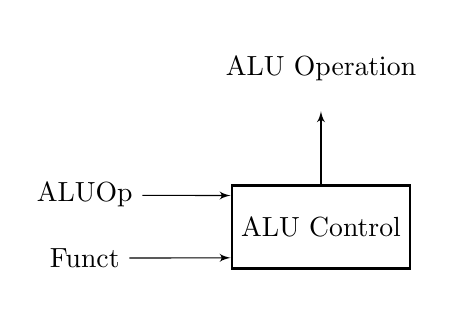
\begin{tikzpicture}
            \node[block] (alucont) at (0,0) {ALU Control};
            \node[empty] (aluop) at (-3, 0.4) {ALUOp};
            \node[empty] (funct) at (-3, -0.4) {Funct};
            \node[empty] (aluope) at (0, 2) {ALU Operation};

            \path[draw, ->] (aluop) -- (alucont.161);
            \path[draw, ->] (funct) -- (alucont.199);
            \path[draw, ->] (alucont) -- (aluope);
        \end{tikzpicture}
    \end{figure}
\end{frame}
\begin{frame}
    The ALU Control starts by looking at the ALUOp from the Control Unit, to
    identify whether or not the instruction is in R-format, in which case it
    should look at the Funct.

    \vspace{\baselineskip}
    In either case, it outputs on the ALU Operation bus, which operation the
    ALU should perform.
\end{frame}
\subsection{Implementation \& Testing}
\begin{frame}
    The SME process should start by looking at the opcode, and have an if on
    whether or not it is in R-format.

    \vspace{\baselineskip}
    In case it is, it should have a \texttt{switch} on the Funct input. If
    it is not, it should have a \texttt{switch} on the opcode. In each case of
    either of the \texttt{switch}s, it should output to the ALU Operation bus.

    \vspace{\baselineskip}
    Note: as always, the source code becomes more readable with a \texttt{enum}
    on the Funct.

    \vspace{\baselineskip}
    The testing is performed in the same manner as with the Control Unit.
\end{frame}

\section{Splitter}
\begin{frame}
    \begin{figure}
        \centering
        \scalebox{0.5}{
            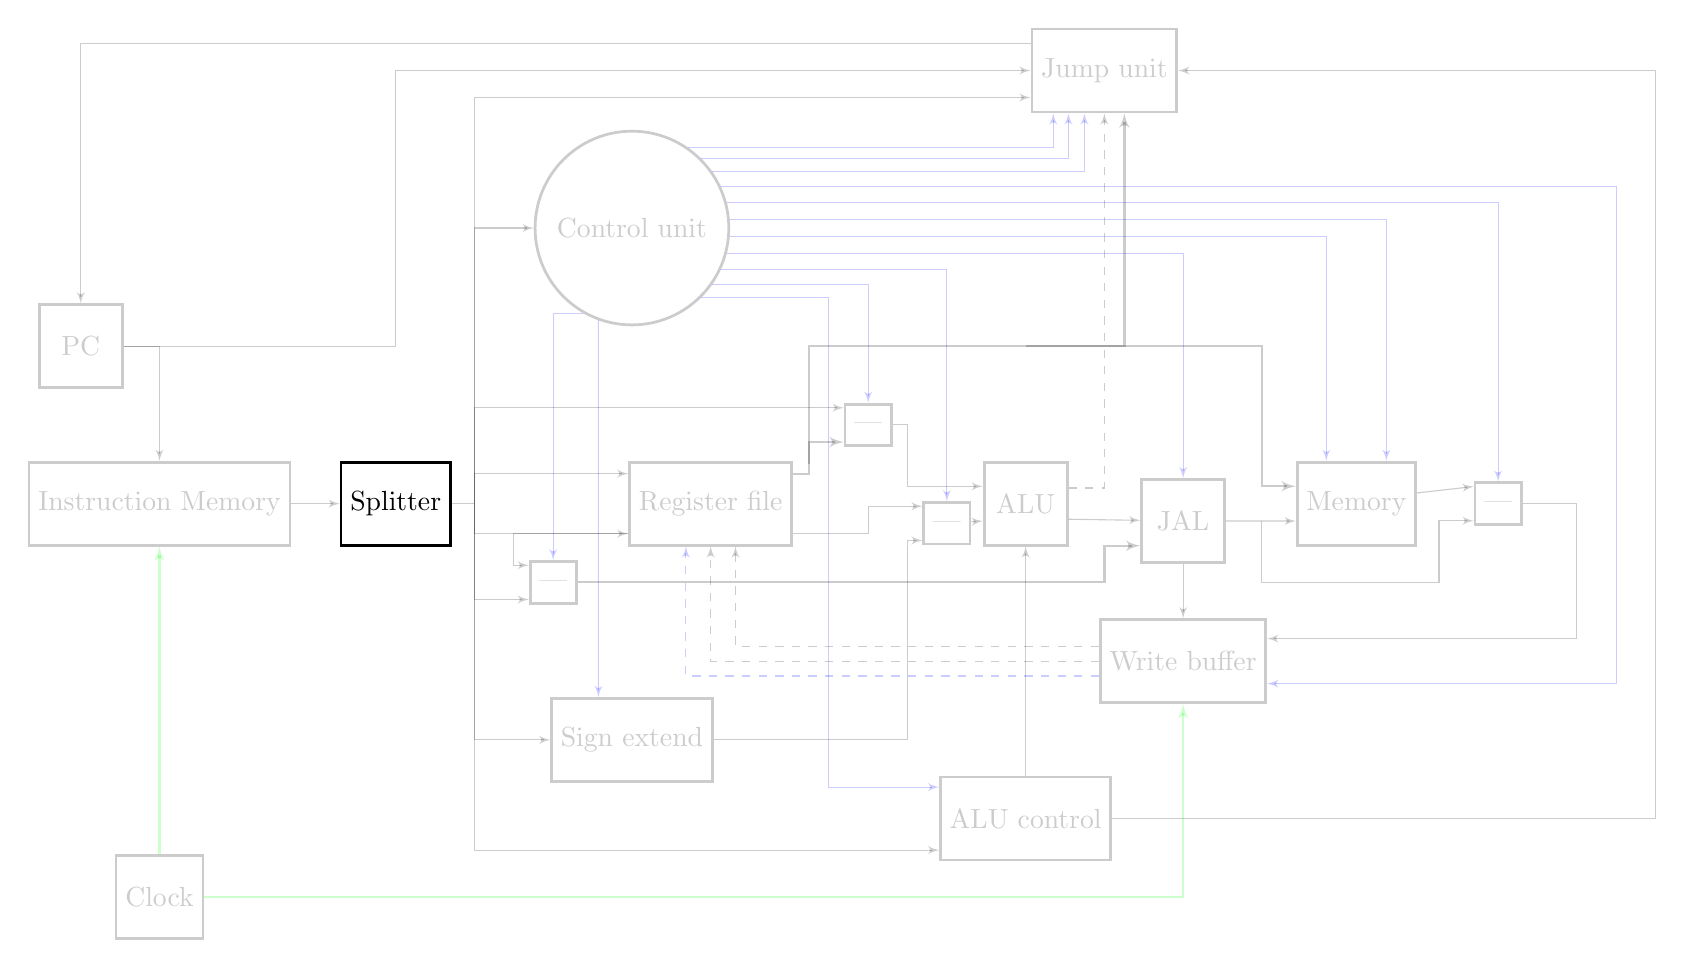
\begin{tikzpicture}
                \node[opacity=0.2,block] (reg) at (0,0) {Register file};
                \node[opacity=0.2,control] (cont) at (-1,3.5) {Control unit};
                \node[opacity=0.2,block] (jump) at (5,5.5) {Jump unit};
                \node[opacity=0.2,empty] (splitspace) at (-3,0) {};
                \node[block] (split) at (-4,0) {Splitter};
                \node[opacity=0.2,block] (if) at (-7,0) {Instruction Memory};
                \node[opacity=0.2,block] (sign) at (-1,-3) {Sign extend};
                \node[opacity=0.2,block] (alu) at (4,0) {ALU};
                \node[opacity=0.2,block] (alucont) at (4,-4) {ALU control};
                \node[opacity=0.2,block] (mem) at (8.2,0) {Memory};
                \node[opacity=0.2,block] (jal) at (6,-0.22) {JAL};
                \node[opacity=0.2,mux] (memread) at (10,0) {|};
                \node[opacity=0.2,mux] (shmt) at (2,1) {|};
                \node[opacity=0.2,mux] (imm) at (3, -0.25) {|};
                \node[opacity=0.2,mux] (regdst) at (-2,-1) {|};
                \node[opacity=0.2,block] (pc) at (-8, 2) {PC};
                \node[opacity=0.2,block] (writebuf) at (6, -2) {Write buffer};

                \path[opacity=0.2,draw, ->] (if) -- (split);
                \path[opacity=0.2,draw, -] (split) -- (splitspace.center);
                \path[opacity=0.2,draw, ->] (splitspace.center) |- (sign);
                \path[opacity=0.2,draw, ->] (splitspace.center) |- (cont);
                \path[opacity=0.2,draw, ->] (splitspace.center) |- (reg.160);
                \path[opacity=0.2,draw, ->] (splitspace.center) |- (reg.200);
                \path[opacity=0.2,draw, ->] (splitspace.center) |- (jump.200);
                \path[opacity=0.2,draw, ->] (splitspace.center) |- (alucont.200);
                \path[opacity=0.2,draw, ->] (splitspace.center) |- (regdst.215);
                \path[opacity=0.2,draw, ->] (splitspace.center) |- (shmt.145);
                \path[opacity=0.2,draw, ->] (reg.200) -| (-2.5, -0.5) |- (regdst.145);
                \path[opacity=0.2,draw, ->] (alucont) -- (alu);
                \path[opacity=0.2,draw, ->] (alucont) -| (12, 0) |- (jump);
                \path[opacity=0.2,draw, ->] (reg.340) -| (2,-0.25) |- (imm.145);
                \path[opacity=0.2,draw, thick, ->] (reg.20) -| (1.25,0.5) |- (shmt.215);
                \path[opacity=0.2,draw, thick, ->] (1.25, 0.5) |- (4, 2) -| (7,1) |- (mem.164);
                \path[opacity=0.2,draw, thick, ->] (4,2) -| (jump.295);
                \path[opacity=0.2,draw, ->] (shmt) -| (2.5, 0.5) |- (alu.158);
                \path[opacity=0.2,draw, dashed, ->] (alu.20) -| (jump);
                \path[opacity=0.2,draw, ->] (alu.340) -- (jal);
                \path[opacity=0.2,draw, ->] (jal) -- (mem.196);
                \path[opacity=0.2,draw, ->] (imm) -- (alu.202);
                \path[opacity=0.2,draw, ->] (7, -0.22) |- (8, -1) -| (9.25,-0.5) |- (memread.215);
                \path[opacity=0.2,draw, ->] (mem.10) -- (memread.145);
                \path[opacity=0.2,draw, ->] (sign) -| (2.5, -1) |- (imm.215);
                \path[opacity=0.2,draw, thick, ->] (regdst) -| (5, -0.6) |- (jal.210);
                \path[opacity=0.2,draw, ->] (pc) -| (if);
                \path[opacity=0.2,draw, ->] (pc) -| (-4, 4) |- (jump);
                \path[opacity=0.2,draw, ->] (jump.160) -| (pc);
                \path[opacity=0.2,draw, ->] (jal) -- (writebuf);
                \path[opacity=0.2,draw, ->] (memread) -| (11, -1) |- (writebuf.15);
                \path[opacity=0.2,draw, dashed, ->] (writebuf.170) -| (reg.300);
                \path[opacity=0.2,draw, dashed, ->] (writebuf) -| (reg);
                \path[opacity=0.2,draw, dashed, ->, color=blue] (writebuf.190) -| (reg.240);

                \path[opacity=0.2,draw, ->, color=blue] (cont.55) -| (jump.220);
                \path[opacity=0.2,draw, ->, color=blue] (cont.45) -| (jump.230);
                \path[opacity=0.2,draw, ->, color=blue] (cont.35) -| (jump.245);
                \path[opacity=0.2,draw, ->, color=blue] (cont.25) -| (11.5,0) |-(writebuf.345);
                \path[opacity=0.2,draw, ->, color=blue] (cont.15) -| (memread);
                \path[opacity=0.2,draw, ->, color=blue] (cont.5) -| (mem.55);
                \path[opacity=0.2,draw, ->, color=blue] (cont.355) -| (mem.125);
                \path[opacity=0.2,draw, ->, color=blue] (cont.345) -| (jal);
                \path[opacity=0.2,draw, ->, color=blue] (cont.335) -| (imm);
                \path[opacity=0.2,draw, ->, color=blue] (cont.325) -| (shmt);
                \path[opacity=0.2,draw, ->, color=blue] (cont.315) -| (1.5, 0.5) |- (alucont.160);
                %\path[opacity=0.2,draw, ->, color=blue] (cont.305) -- (reg.110);
                \path[opacity=0.2,draw, ->, color=blue] (cont.250) -- (sign.128);
                \path[opacity=0.2,draw, ->, color=blue] (cont.240) -| (regdst);

                \node[opacity=0.2,block] (clock) at (-7, -5) {Clock};
                \path[opacity=0.2,draw, ->, thick, color=green] (clock) -- (if);
                \path[opacity=0.2,draw, ->, thick, color=green] (clock) -| (writebuf);
            \end{tikzpicture}
        }
    \end{figure}
\end{frame}
\subsection{Background}
\begin{frame}
    The Splitter is a very simple component. It takes the instruction read from
    memory, and splits it up onto multiple busses. It has one input:
    \begin{itemize}
        \item Instruction
    \end{itemize}
    and it produces 6 outputs (bit numbers are inclusive):
    \begin{itemize}
        \item Opcode - bits 26-31
        \item Read Address A - bits 21-25
        \item Read Address B - bits 16-20
        \item Write Address - bits 11-15
        \item Immediate - bits 0-15
        \item Funct - bits 0-5
    \end{itemize}
\end{frame}
\begin{frame}
    \begin{figure}
        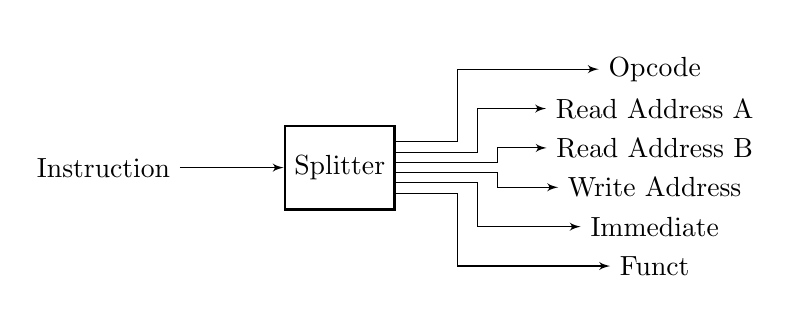
\begin{tikzpicture}
            \node[block] (split) at (0,0) {Splitter};
            \node[empty] (inst) at (-3,0) {Instruction};
            \node[empty] (op) at (4,1.25) {Opcode};
            \node[empty] (ra) at (4,0.75) {Read Address A};
            \node[empty] (rb) at (4,0.25) {Read Address B};
            \node[empty] (wa) at (4,-0.25) {Write Address};
            \node[empty] (imm) at (4,-0.75) {Immediate};
            \node[empty] (fun) at (4,-1.25) {Funct};

            \path[draw, ->] (inst) -- (split);
            \path[draw, ->] (split.25) -| (1.5, 1) |- (op);
            \path[draw, ->] (split.15) -| (1.75,0.5) |- (ra);
            \path[draw, ->] (split.5) -| (2,0.125) |- (rb);
            \path[draw, ->] (split.355) -| (2,-0.125) |- (wa);
            \path[draw, ->] (split.345) -| (1.75,-0.5) |- (imm);
            \path[draw, ->] (split.335) -| (1.5, -1) |- (fun);
        \end{tikzpicture}
    \end{figure}
\end{frame}
\subsection{Implementation \& Testing}
\begin{frame}
    Implementing the Splitter in SME is very simple. We just take the
    instruction, and use C\# bit hacking to extract the bits that we need, and
    send the result out on the corresponding busses.

    \vspace{\baselineskip}
    As always, testing is done by constructing a tester process, which sends
    input to the Splitter, and which verifies the output from the Splitter.
\end{frame}

\section{Sign Extend}
\begin{frame}
    \begin{figure}
        \centering
        \scalebox{0.5}{
            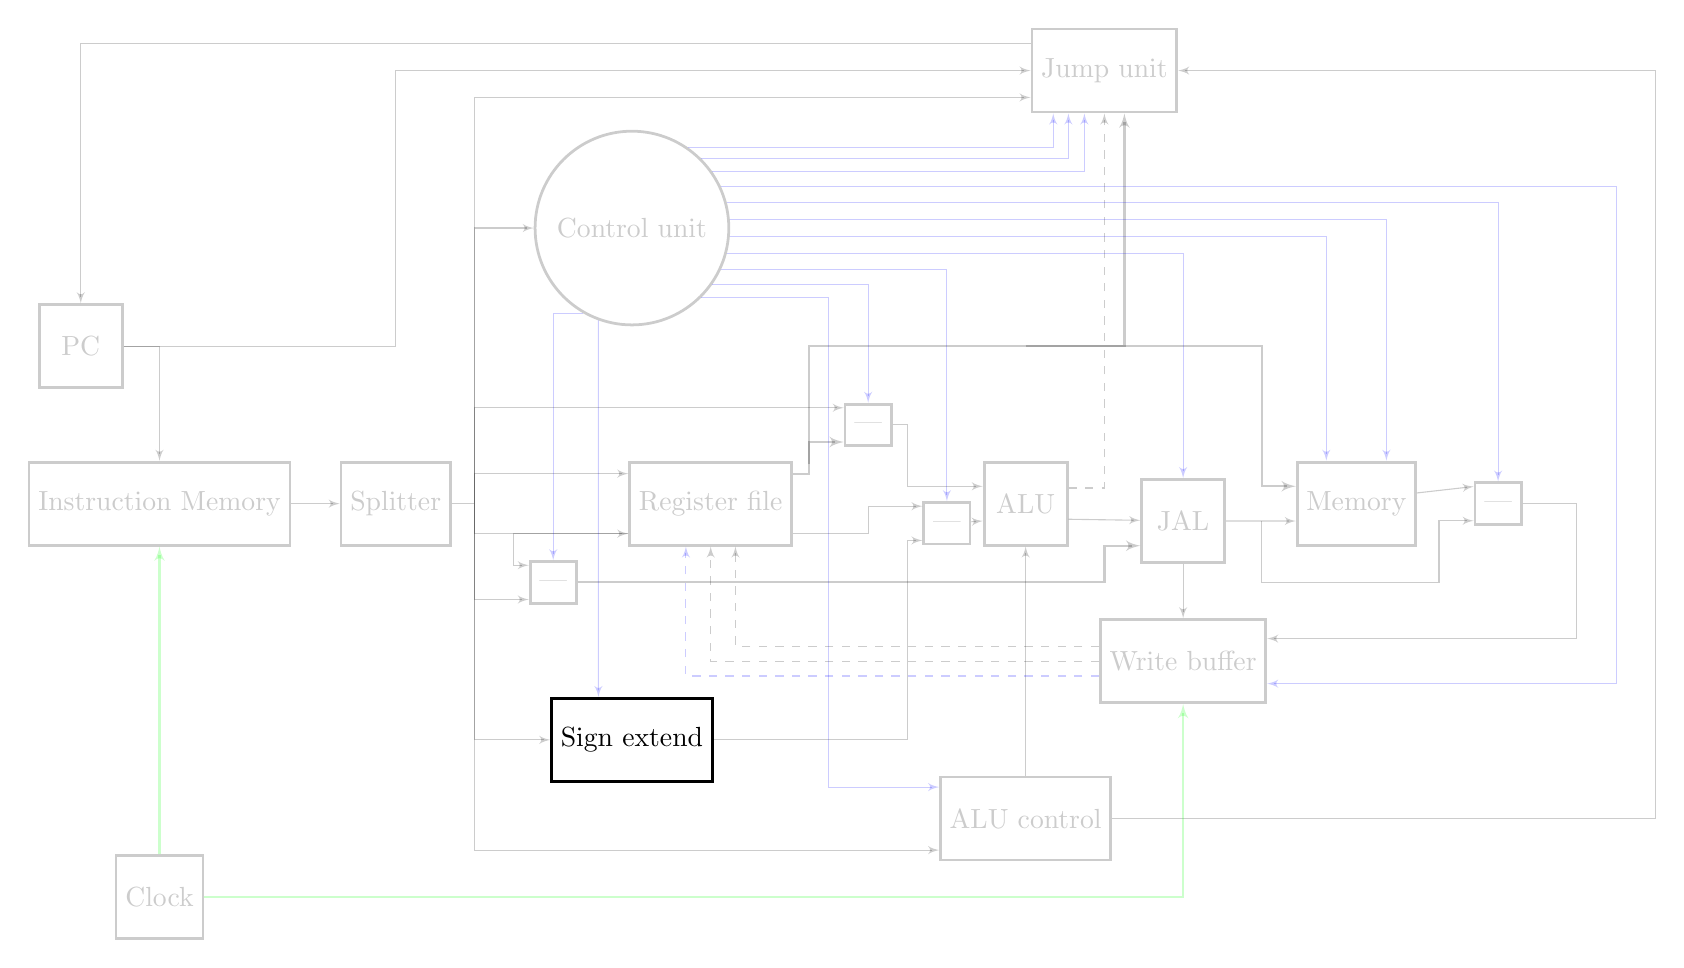
\begin{tikzpicture}
                \node[opacity=0.2,block] (reg) at (0,0) {Register file};
                \node[opacity=0.2,control] (cont) at (-1,3.5) {Control unit};
                \node[opacity=0.2,block] (jump) at (5,5.5) {Jump unit};
                \node[opacity=0.2,empty] (splitspace) at (-3,0) {};
                \node[opacity=0.2,block] (split) at (-4,0) {Splitter};
                \node[opacity=0.2,block] (if) at (-7,0) {Instruction Memory};
                \node[block] (sign) at (-1,-3) {Sign extend};
                \node[opacity=0.2,block] (alu) at (4,0) {ALU};
                \node[opacity=0.2,block] (alucont) at (4,-4) {ALU control};
                \node[opacity=0.2,block] (mem) at (8.2,0) {Memory};
                \node[opacity=0.2,block] (jal) at (6,-0.22) {JAL};
                \node[opacity=0.2,mux] (memread) at (10,0) {|};
                \node[opacity=0.2,mux] (shmt) at (2,1) {|};
                \node[opacity=0.2,mux] (imm) at (3, -0.25) {|};
                \node[opacity=0.2,mux] (regdst) at (-2,-1) {|};
                \node[opacity=0.2,block] (pc) at (-8, 2) {PC};
                \node[opacity=0.2,block] (writebuf) at (6, -2) {Write buffer};

                \path[opacity=0.2,draw, ->] (if) -- (split);
                \path[opacity=0.2,draw, -] (split) -- (splitspace.center);
                \path[opacity=0.2,draw, ->] (splitspace.center) |- (sign);
                \path[opacity=0.2,draw, ->] (splitspace.center) |- (cont);
                \path[opacity=0.2,draw, ->] (splitspace.center) |- (reg.160);
                \path[opacity=0.2,draw, ->] (splitspace.center) |- (reg.200);
                \path[opacity=0.2,draw, ->] (splitspace.center) |- (jump.200);
                \path[opacity=0.2,draw, ->] (splitspace.center) |- (alucont.200);
                \path[opacity=0.2,draw, ->] (splitspace.center) |- (regdst.215);
                \path[opacity=0.2,draw, ->] (splitspace.center) |- (shmt.145);
                \path[opacity=0.2,draw, ->] (reg.200) -| (-2.5, -0.5) |- (regdst.145);
                \path[opacity=0.2,draw, ->] (alucont) -- (alu);
                \path[opacity=0.2,draw, ->] (alucont) -| (12, 0) |- (jump);
                \path[opacity=0.2,draw, ->] (reg.340) -| (2,-0.25) |- (imm.145);
                \path[opacity=0.2,draw, thick, ->] (reg.20) -| (1.25,0.5) |- (shmt.215);
                \path[opacity=0.2,draw, thick, ->] (1.25, 0.5) |- (4, 2) -| (7,1) |- (mem.164);
                \path[opacity=0.2,draw, thick, ->] (4,2) -| (jump.295);
                \path[opacity=0.2,draw, ->] (shmt) -| (2.5, 0.5) |- (alu.158);
                \path[opacity=0.2,draw, dashed, ->] (alu.20) -| (jump);
                \path[opacity=0.2,draw, ->] (alu.340) -- (jal);
                \path[opacity=0.2,draw, ->] (jal) -- (mem.196);
                \path[opacity=0.2,draw, ->] (imm) -- (alu.202);
                \path[opacity=0.2,draw, ->] (7, -0.22) |- (8, -1) -| (9.25,-0.5) |- (memread.215);
                \path[opacity=0.2,draw, ->] (mem.10) -- (memread.145);
                \path[opacity=0.2,draw, ->] (sign) -| (2.5, -1) |- (imm.215);
                \path[opacity=0.2,draw, thick, ->] (regdst) -| (5, -0.6) |- (jal.210);
                \path[opacity=0.2,draw, ->] (pc) -| (if);
                \path[opacity=0.2,draw, ->] (pc) -| (-4, 4) |- (jump);
                \path[opacity=0.2,draw, ->] (jump.160) -| (pc);
                \path[opacity=0.2,draw, ->] (jal) -- (writebuf);
                \path[opacity=0.2,draw, ->] (memread) -| (11, -1) |- (writebuf.15);
                \path[opacity=0.2,draw, dashed, ->] (writebuf.170) -| (reg.300);
                \path[opacity=0.2,draw, dashed, ->] (writebuf) -| (reg);
                \path[opacity=0.2,draw, dashed, ->, color=blue] (writebuf.190) -| (reg.240);

                \path[opacity=0.2,draw, ->, color=blue] (cont.55) -| (jump.220);
                \path[opacity=0.2,draw, ->, color=blue] (cont.45) -| (jump.230);
                \path[opacity=0.2,draw, ->, color=blue] (cont.35) -| (jump.245);
                \path[opacity=0.2,draw, ->, color=blue] (cont.25) -| (11.5,0) |-(writebuf.345);
                \path[opacity=0.2,draw, ->, color=blue] (cont.15) -| (memread);
                \path[opacity=0.2,draw, ->, color=blue] (cont.5) -| (mem.55);
                \path[opacity=0.2,draw, ->, color=blue] (cont.355) -| (mem.125);
                \path[opacity=0.2,draw, ->, color=blue] (cont.345) -| (jal);
                \path[opacity=0.2,draw, ->, color=blue] (cont.335) -| (imm);
                \path[opacity=0.2,draw, ->, color=blue] (cont.325) -| (shmt);
                \path[opacity=0.2,draw, ->, color=blue] (cont.315) -| (1.5, 0.5) |- (alucont.160);
                %\path[opacity=0.2,draw, ->, color=blue] (cont.305) -- (reg.110);
                \path[opacity=0.2,draw, ->, color=blue] (cont.250) -- (sign.128);
                \path[opacity=0.2,draw, ->, color=blue] (cont.240) -| (regdst);

                \node[opacity=0.2,block] (clock) at (-7, -5) {Clock};
                \path[opacity=0.2,draw, ->, thick, color=green] (clock) -- (if);
                \path[opacity=0.2,draw, ->, thick, color=green] (clock) -| (writebuf);
            \end{tikzpicture}
        }
    \end{figure}
\end{frame}
\subsection{Background}
\begin{frame}
    The Sign Extend is used for extracting values from the instruction. It
    takes its input, which is 16-bit, and converts it into a 32-bit value,
    extending the sign if present. It takes one 16-bit input:
    \begin{itemize}
        \item Immediate
    \end{itemize}
    and produces one 32-bit output:
    \begin{itemize}
        \item Sign extended immediate
    \end{itemize}
\end{frame}
\begin{frame}
    \begin{figure}
        
\begin{tikzpicture}
            \node[block] (sign) at (0,0) {Sign Extend};
            \node[empty] (imm) at (-3,0) {Immediate};
            \node[empty] (immout) at (4,0) {Sign extended immediate};

            \path[draw, ->] (imm) -- (sign);
            \path[draw, ->] (sign) -- (immout);
        \end{tikzpicture}
    \end{figure}
\end{frame}
\subsection{Implementation \& Testing}
\begin{frame}
    The SME process takes the 16-bit immediate as input. Upon receiving all of
    its input, it outputs the input on its 32-bit output bus. In this case, C\#
    handles the extending for us.

    \vspace{\baselineskip}
    The testing is analogous to the previous tests.

    \vspace{\baselineskip}
    Note: It is an good idea to test both negative and positive numbers.
\end{frame}

\section{Instruction Memory}
\begin{frame}
    \begin{figure}
        \centering
        \scalebox{0.5}{
            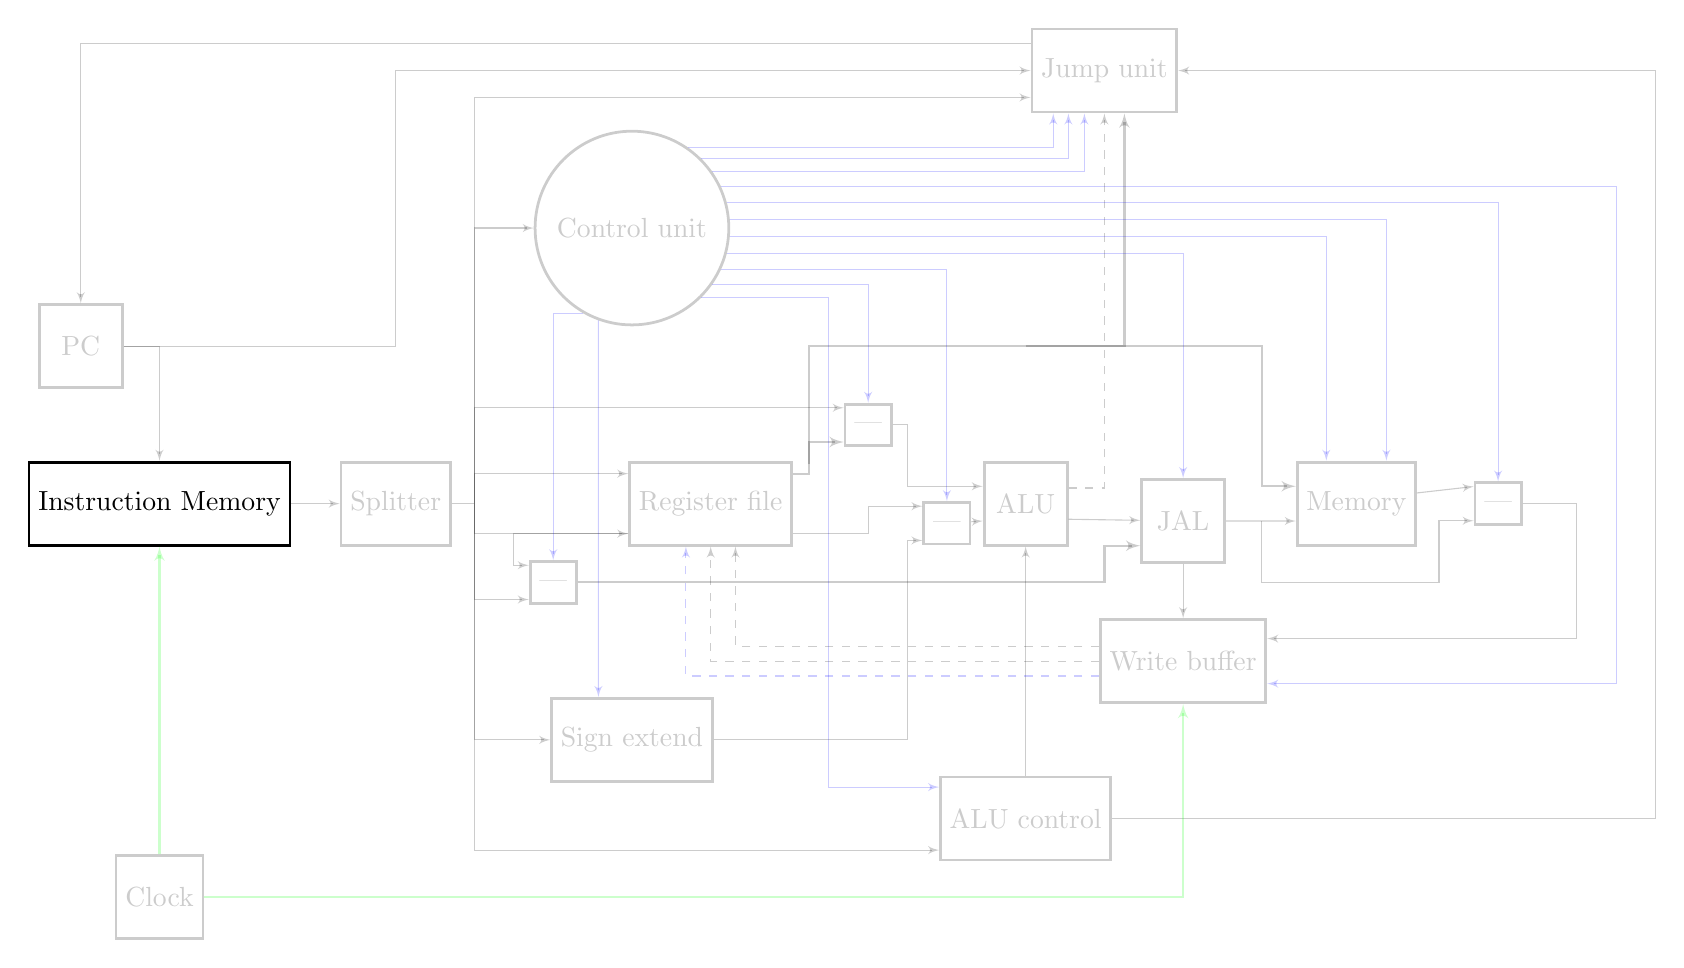
\begin{tikzpicture}
                \node[opacity=0.2,block] (reg) at (0,0) {Register file};
                \node[opacity=0.2,control] (cont) at (-1,3.5) {Control unit};
                \node[opacity=0.2,block] (jump) at (5,5.5) {Jump unit};
                \node[opacity=0.2,empty] (splitspace) at (-3,0) {};
                \node[opacity=0.2,block] (split) at (-4,0) {Splitter};
                \node[block] (if) at (-7,0) {Instruction Memory};
                \node[opacity=0.2,block] (sign) at (-1,-3) {Sign extend};
                \node[opacity=0.2,block] (alu) at (4,0) {ALU};
                \node[opacity=0.2,block] (alucont) at (4,-4) {ALU control};
                \node[opacity=0.2,block] (mem) at (8.2,0) {Memory};
                \node[opacity=0.2,block] (jal) at (6,-0.22) {JAL};
                \node[opacity=0.2,mux] (memread) at (10,0) {|};
                \node[opacity=0.2,mux] (shmt) at (2,1) {|};
                \node[opacity=0.2,mux] (imm) at (3, -0.25) {|};
                \node[opacity=0.2,mux] (regdst) at (-2,-1) {|};
                \node[opacity=0.2,block] (pc) at (-8, 2) {PC};
                \node[opacity=0.2,block] (writebuf) at (6, -2) {Write buffer};

                \path[opacity=0.2,draw, ->] (if) -- (split);
                \path[opacity=0.2,draw, -] (split) -- (splitspace.center);
                \path[opacity=0.2,draw, ->] (splitspace.center) |- (sign);
                \path[opacity=0.2,draw, ->] (splitspace.center) |- (cont);
                \path[opacity=0.2,draw, ->] (splitspace.center) |- (reg.160);
                \path[opacity=0.2,draw, ->] (splitspace.center) |- (reg.200);
                \path[opacity=0.2,draw, ->] (splitspace.center) |- (jump.200);
                \path[opacity=0.2,draw, ->] (splitspace.center) |- (alucont.200);
                \path[opacity=0.2,draw, ->] (splitspace.center) |- (regdst.215);
                \path[opacity=0.2,draw, ->] (splitspace.center) |- (shmt.145);
                \path[opacity=0.2,draw, ->] (reg.200) -| (-2.5, -0.5) |- (regdst.145);
                \path[opacity=0.2,draw, ->] (alucont) -- (alu);
                \path[opacity=0.2,draw, ->] (alucont) -| (12, 0) |- (jump);
                \path[opacity=0.2,draw, ->] (reg.340) -| (2,-0.25) |- (imm.145);
                \path[opacity=0.2,draw, thick, ->] (reg.20) -| (1.25,0.5) |- (shmt.215);
                \path[opacity=0.2,draw, thick, ->] (1.25, 0.5) |- (4, 2) -| (7,1) |- (mem.164);
                \path[opacity=0.2,draw, thick, ->] (4,2) -| (jump.295);
                \path[opacity=0.2,draw, ->] (shmt) -| (2.5, 0.5) |- (alu.158);
                \path[opacity=0.2,draw, dashed, ->] (alu.20) -| (jump);
                \path[opacity=0.2,draw, ->] (alu.340) -- (jal);
                \path[opacity=0.2,draw, ->] (jal) -- (mem.196);
                \path[opacity=0.2,draw, ->] (imm) -- (alu.202);
                \path[opacity=0.2,draw, ->] (7, -0.22) |- (8, -1) -| (9.25,-0.5) |- (memread.215);
                \path[opacity=0.2,draw, ->] (mem.10) -- (memread.145);
                \path[opacity=0.2,draw, ->] (sign) -| (2.5, -1) |- (imm.215);
                \path[opacity=0.2,draw, thick, ->] (regdst) -| (5, -0.6) |- (jal.210);
                \path[opacity=0.2,draw, ->] (pc) -| (if);
                \path[opacity=0.2,draw, ->] (pc) -| (-4, 4) |- (jump);
                \path[opacity=0.2,draw, ->] (jump.160) -| (pc);
                \path[opacity=0.2,draw, ->] (jal) -- (writebuf);
                \path[opacity=0.2,draw, ->] (memread) -| (11, -1) |- (writebuf.15);
                \path[opacity=0.2,draw, dashed, ->] (writebuf.170) -| (reg.300);
                \path[opacity=0.2,draw, dashed, ->] (writebuf) -| (reg);
                \path[opacity=0.2,draw, dashed, ->, color=blue] (writebuf.190) -| (reg.240);

                \path[opacity=0.2,draw, ->, color=blue] (cont.55) -| (jump.220);
                \path[opacity=0.2,draw, ->, color=blue] (cont.45) -| (jump.230);
                \path[opacity=0.2,draw, ->, color=blue] (cont.35) -| (jump.245);
                \path[opacity=0.2,draw, ->, color=blue] (cont.25) -| (11.5,0) |-(writebuf.345);
                \path[opacity=0.2,draw, ->, color=blue] (cont.15) -| (memread);
                \path[opacity=0.2,draw, ->, color=blue] (cont.5) -| (mem.55);
                \path[opacity=0.2,draw, ->, color=blue] (cont.355) -| (mem.125);
                \path[opacity=0.2,draw, ->, color=blue] (cont.345) -| (jal);
                \path[opacity=0.2,draw, ->, color=blue] (cont.335) -| (imm);
                \path[opacity=0.2,draw, ->, color=blue] (cont.325) -| (shmt);
                \path[opacity=0.2,draw, ->, color=blue] (cont.315) -| (1.5, 0.5) |- (alucont.160);
                %\path[opacity=0.2,draw, ->, color=blue] (cont.305) -- (reg.110);
                \path[opacity=0.2,draw, ->, color=blue] (cont.250) -- (sign.128);
                \path[opacity=0.2,draw, ->, color=blue] (cont.240) -| (regdst);

                \node[opacity=0.2,block] (clock) at (-7, -5) {Clock};
                \path[opacity=0.2,draw, ->, thick, color=green] (clock) -- (if);
                \path[opacity=0.2,draw, ->, thick, color=green] (clock) -| (writebuf);
            \end{tikzpicture}
        }
    \end{figure}
\end{frame}
\subsection{Background}
\begin{frame}
    The Instruction Memory is the part of the processor, which holds the
    program. It has a chunk of memory, and for each clock, it outputs the
    memory at the given address. It has one input:
    \begin{itemize}
        \item Program Counter
    \end{itemize}
    and it produces one output:
    \begin{itemize}
        \item Instruction
    \end{itemize}
\end{frame}
\begin{frame}
    \begin{figure}
        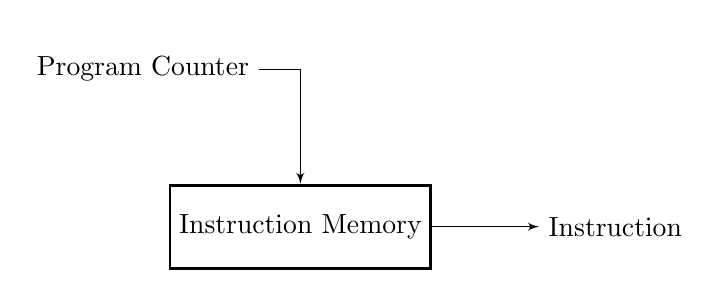
\begin{tikzpicture}
            \node[block] (inmem) at (0,0) {Instruction Memory};
            \node[empty] (pc) at (-2, 2) {Program Counter};
            \node[empty] (inst) at (4,0) {Instruction};

            \path[draw, ->] (pc) -| (inmem);
            \path[draw, ->] (inmem) -- (inst);
        \end{tikzpicture}
    \end{figure}
\end{frame}
\subsection{Implementation \& Testing}
\begin{frame}
    Upon receiving all of its inputs, the Instruction Memory reads the address
    from the Program Counter bus, and outputs the value within its memory at
    the read address, on the instruction bus.

    \vspace{\baselineskip}
    Usually memory should be a byte array. However, since we are working with
    C\#, we can just use a \texttt{int} array for now, as then we dont have to
    worry about word alignment for now.

    \vspace{\baselineskip}
    The Instruction Memory is tested by having a tester process, which inputs
    some reading addresses, and verifies whether or not they are as expected.

    \vspace{\baselineskip}
    Note: since there is no way to input a program into the Instruction Memory,
    the program should be hardcoded for now.
\end{frame}

\section{Memory Unit}
\begin{frame}
    \begin{figure}
        \centering
        \scalebox{0.5}{
            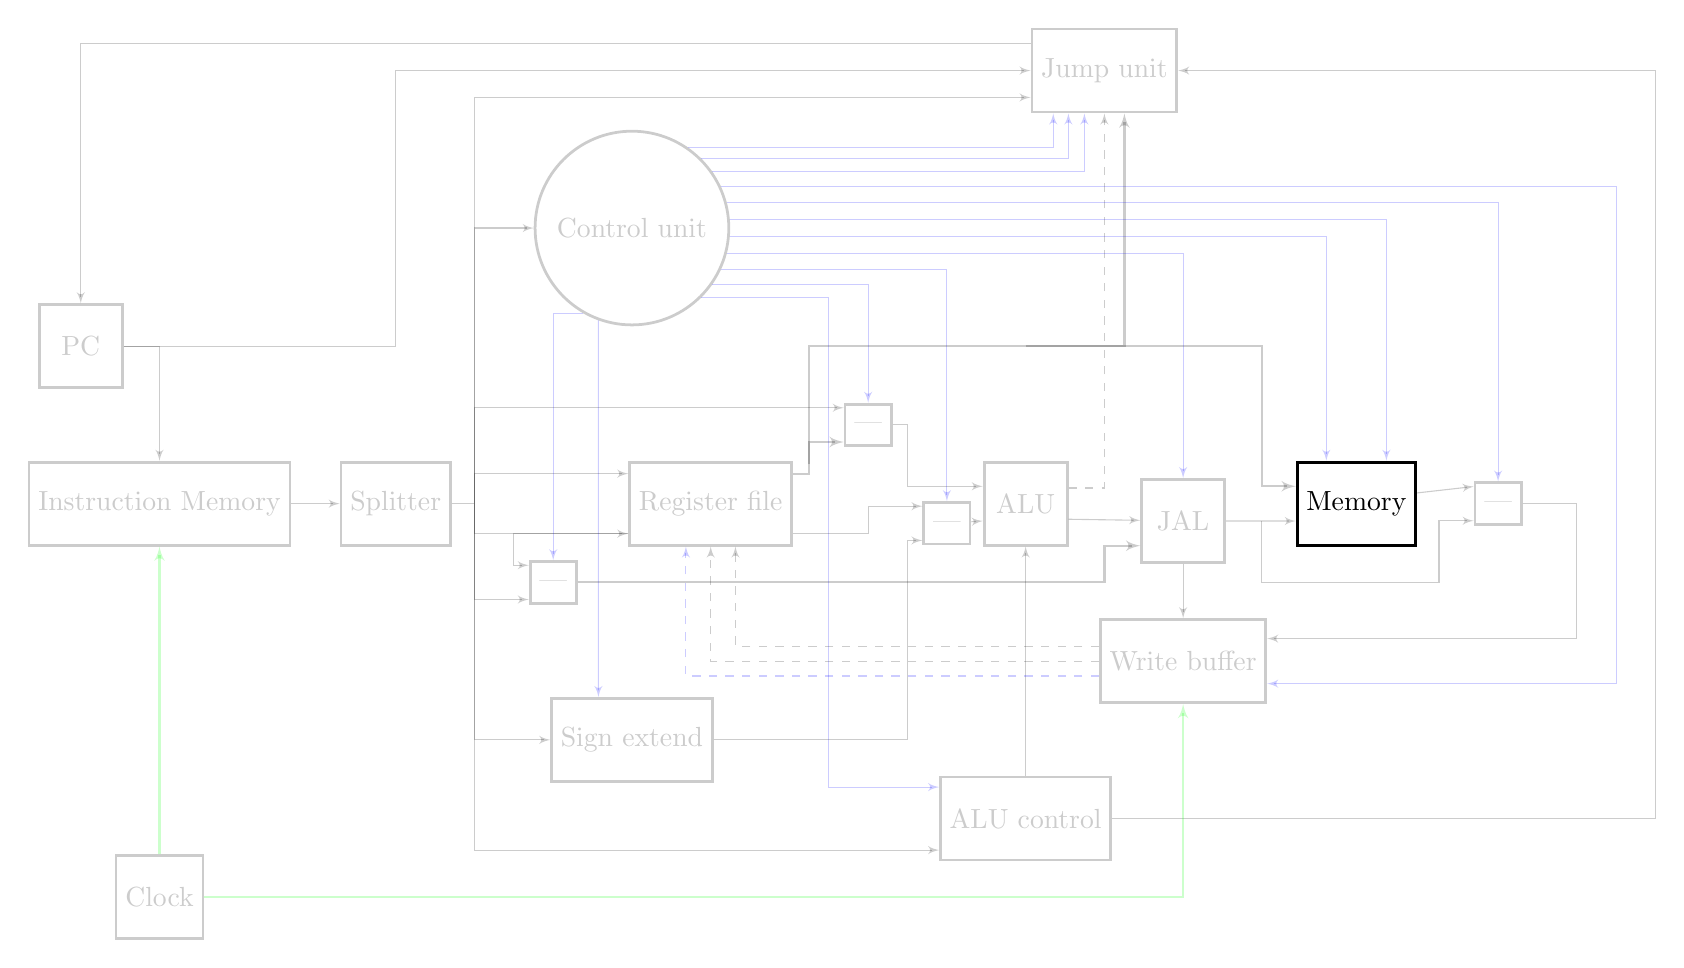
\begin{tikzpicture}
                \node[opacity=0.2,block] (reg) at (0,0) {Register file};
                \node[opacity=0.2,control] (cont) at (-1,3.5) {Control unit};
                \node[opacity=0.2,block] (jump) at (5,5.5) {Jump unit};
                \node[opacity=0.2,empty] (splitspace) at (-3,0) {};
                \node[opacity=0.2,block] (split) at (-4,0) {Splitter};
                \node[opacity=0.2,block] (if) at (-7,0) {Instruction Memory};
                \node[opacity=0.2,block] (sign) at (-1,-3) {Sign extend};
                \node[opacity=0.2,block] (alu) at (4,0) {ALU};
                \node[opacity=0.2,block] (alucont) at (4,-4) {ALU control};
                \node[block] (mem) at (8.2,0) {Memory};
                \node[opacity=0.2,block] (jal) at (6,-0.22) {JAL};
                \node[opacity=0.2,mux] (memread) at (10,0) {|};
                \node[opacity=0.2,mux] (shmt) at (2,1) {|};
                \node[opacity=0.2,mux] (imm) at (3, -0.25) {|};
                \node[opacity=0.2,mux] (regdst) at (-2,-1) {|};
                \node[opacity=0.2,block] (pc) at (-8, 2) {PC};
                \node[opacity=0.2,block] (writebuf) at (6, -2) {Write buffer};

                \path[opacity=0.2,draw, ->] (if) -- (split);
                \path[opacity=0.2,draw, -] (split) -- (splitspace.center);
                \path[opacity=0.2,draw, ->] (splitspace.center) |- (sign);
                \path[opacity=0.2,draw, ->] (splitspace.center) |- (cont);
                \path[opacity=0.2,draw, ->] (splitspace.center) |- (reg.160);
                \path[opacity=0.2,draw, ->] (splitspace.center) |- (reg.200);
                \path[opacity=0.2,draw, ->] (splitspace.center) |- (jump.200);
                \path[opacity=0.2,draw, ->] (splitspace.center) |- (alucont.200);
                \path[opacity=0.2,draw, ->] (splitspace.center) |- (regdst.215);
                \path[opacity=0.2,draw, ->] (splitspace.center) |- (shmt.145);
                \path[opacity=0.2,draw, ->] (reg.200) -| (-2.5, -0.5) |- (regdst.145);
                \path[opacity=0.2,draw, ->] (alucont) -- (alu);
                \path[opacity=0.2,draw, ->] (alucont) -| (12, 0) |- (jump);
                \path[opacity=0.2,draw, ->] (reg.340) -| (2,-0.25) |- (imm.145);
                \path[opacity=0.2,draw, thick, ->] (reg.20) -| (1.25,0.5) |- (shmt.215);
                \path[opacity=0.2,draw, thick, ->] (1.25, 0.5) |- (4, 2) -| (7,1) |- (mem.164);
                \path[opacity=0.2,draw, thick, ->] (4,2) -| (jump.295);
                \path[opacity=0.2,draw, ->] (shmt) -| (2.5, 0.5) |- (alu.158);
                \path[opacity=0.2,draw, dashed, ->] (alu.20) -| (jump);
                \path[opacity=0.2,draw, ->] (alu.340) -- (jal);
                \path[opacity=0.2,draw, ->] (jal) -- (mem.196);
                \path[opacity=0.2,draw, ->] (imm) -- (alu.202);
                \path[opacity=0.2,draw, ->] (7, -0.22) |- (8, -1) -| (9.25,-0.5) |- (memread.215);
                \path[opacity=0.2,draw, ->] (mem.10) -- (memread.145);
                \path[opacity=0.2,draw, ->] (sign) -| (2.5, -1) |- (imm.215);
                \path[opacity=0.2,draw, thick, ->] (regdst) -| (5, -0.6) |- (jal.210);
                \path[opacity=0.2,draw, ->] (pc) -| (if);
                \path[opacity=0.2,draw, ->] (pc) -| (-4, 4) |- (jump);
                \path[opacity=0.2,draw, ->] (jump.160) -| (pc);
                \path[opacity=0.2,draw, ->] (jal) -- (writebuf);
                \path[opacity=0.2,draw, ->] (memread) -| (11, -1) |- (writebuf.15);
                \path[opacity=0.2,draw, dashed, ->] (writebuf.170) -| (reg.300);
                \path[opacity=0.2,draw, dashed, ->] (writebuf) -| (reg);
                \path[opacity=0.2,draw, dashed, ->, color=blue] (writebuf.190) -| (reg.240);

                \path[opacity=0.2,draw, ->, color=blue] (cont.55) -| (jump.220);
                \path[opacity=0.2,draw, ->, color=blue] (cont.45) -| (jump.230);
                \path[opacity=0.2,draw, ->, color=blue] (cont.35) -| (jump.245);
                \path[opacity=0.2,draw, ->, color=blue] (cont.25) -| (11.5,0) |-(writebuf.345);
                \path[opacity=0.2,draw, ->, color=blue] (cont.15) -| (memread);
                \path[opacity=0.2,draw, ->, color=blue] (cont.5) -| (mem.55);
                \path[opacity=0.2,draw, ->, color=blue] (cont.355) -| (mem.125);
                \path[opacity=0.2,draw, ->, color=blue] (cont.345) -| (jal);
                \path[opacity=0.2,draw, ->, color=blue] (cont.335) -| (imm);
                \path[opacity=0.2,draw, ->, color=blue] (cont.325) -| (shmt);
                \path[opacity=0.2,draw, ->, color=blue] (cont.315) -| (1.5, 0.5) |- (alucont.160);
                %\path[opacity=0.2,draw, ->, color=blue] (cont.305) -- (reg.110);
                \path[opacity=0.2,draw, ->, color=blue] (cont.250) -- (sign.128);
                \path[opacity=0.2,draw, ->, color=blue] (cont.240) -| (regdst);

                \node[opacity=0.2,block] (clock) at (-7, -5) {Clock};
                \path[opacity=0.2,draw, ->, thick, color=green] (clock) -- (if);
                \path[opacity=0.2,draw, ->, thick, color=green] (clock) -| (writebuf);
            \end{tikzpicture}
        }
    \end{figure}
\end{frame}
\subsection{Background}
\begin{frame}
    The Memory Unit is the main memory. It can either be written to or read
    from. The values from and to the memory are word sized, i.e. in the 32-bit
    processor, the word size is 32. It takes four inputs:
    \begin{itemize}
        \item Address
        \item Data
        \item \texttt{MemRead}
        \item \texttt{MemWrite}
    \end{itemize}
    and produces one output:
    \begin{itemize}
        \item Read Data
    \end{itemize}
\end{frame}
\begin{frame}
    \begin{figure}
        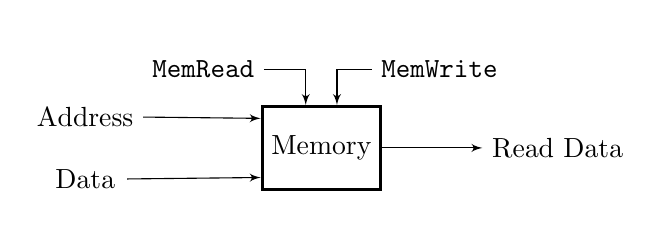
\begin{tikzpicture}
            \node[block] (mem) at (0,0) {Memory};
            \node[empty] (addr) at (-3,0.4) {Address};
            \node[empty] (data) at (-3,-0.4) {Data};
            \node[empty] (memread) at (-1.5, 1) {\texttt{MemRead}};
            \node[empty] (memwrite) at (1.5, 1) {\texttt{MemWrite}};
            \node[empty] (readdata) at (3, 0) {Read Data};

            \path[draw, ->] (addr) -- (mem.154);
            \path[draw, ->] (data) -- (mem.206);
            \path[draw, ->] (memread) -| (mem.110);
            \path[draw, ->] (memwrite) -| (mem.70);
            \path[draw, ->] (mem) -- (readdata);
        \end{tikzpicture}
    \end{figure}
\end{frame}
\subsection{Implementation \& Testing}
\begin{frame}
    The memory should be implemented as a \texttt{byte} array, as this makes it
    easier later on when running programs on the processor. It should pack 4
    bytes into an \texttt{int} value.

    \vspace{\baselineskip}
    Upon receiving all of its inputs, the SME process should first check if it
    should read, in which case it should just output the value stored at the
    address of the Address bus. Then it needs to check whether or not it should
    write, in which case it should write the value from the Data bus into the
    memory at the given address.

    \vspace{\baselineskip}
    The Memory is tested in the same manner as the Register File.
\end{frame}

\section{Write Back}
\begin{frame}
    \begin{figure}
        \centering
        \scalebox{0.5}{
            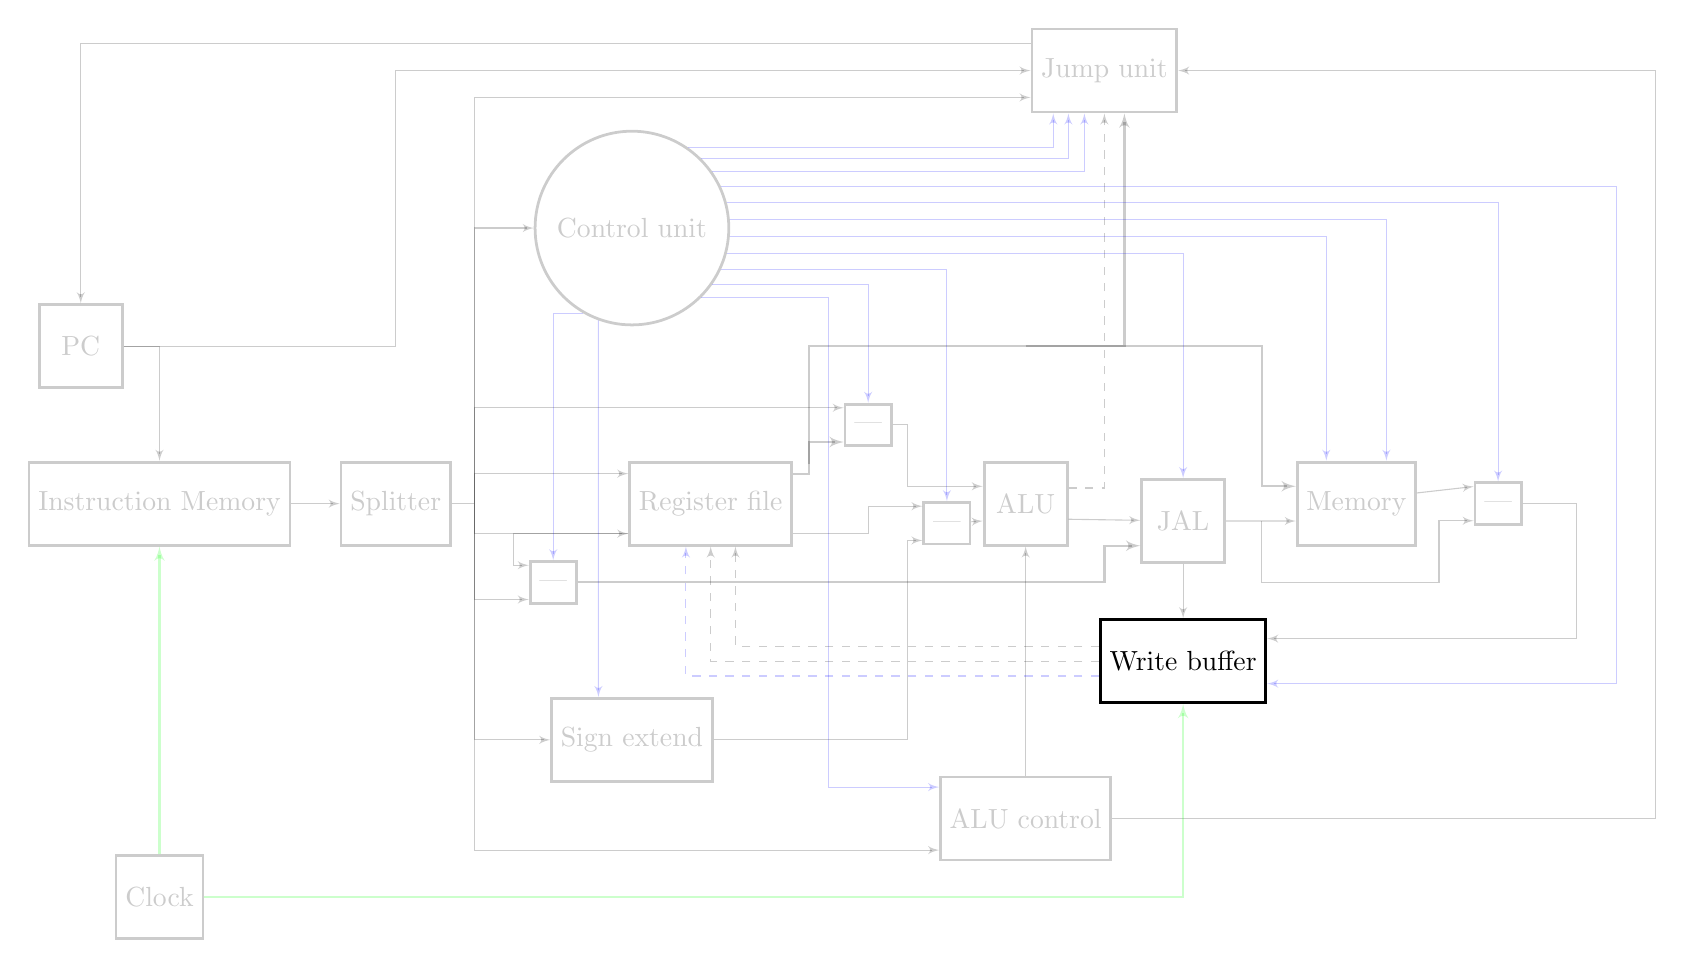
\begin{tikzpicture}
                \node[opacity=0.2,block] (reg) at (0,0) {Register file};
                \node[opacity=0.2,control] (cont) at (-1,3.5) {Control unit};
                \node[opacity=0.2,block] (jump) at (5,5.5) {Jump unit};
                \node[opacity=0.2,empty] (splitspace) at (-3,0) {};
                \node[opacity=0.2,block] (split) at (-4,0) {Splitter};
                \node[opacity=0.2,block] (if) at (-7,0) {Instruction Memory};
                \node[opacity=0.2,block] (sign) at (-1,-3) {Sign extend};
                \node[opacity=0.2,block] (alu) at (4,0) {ALU};
                \node[opacity=0.2,block] (alucont) at (4,-4) {ALU control};
                \node[opacity=0.2,block] (mem) at (8.2,0) {Memory};
                \node[opacity=0.2,block] (jal) at (6,-0.22) {JAL};
                \node[opacity=0.2,mux] (memread) at (10,0) {|};
                \node[opacity=0.2,mux] (shmt) at (2,1) {|};
                \node[opacity=0.2,mux] (imm) at (3, -0.25) {|};
                \node[opacity=0.2,mux] (regdst) at (-2,-1) {|};
                \node[opacity=0.2,block] (pc) at (-8, 2) {PC};
                \node[block] (writebuf) at (6, -2) {Write buffer};

                \path[opacity=0.2,draw, ->] (if) -- (split);
                \path[opacity=0.2,draw, -] (split) -- (splitspace.center);
                \path[opacity=0.2,draw, ->] (splitspace.center) |- (sign);
                \path[opacity=0.2,draw, ->] (splitspace.center) |- (cont);
                \path[opacity=0.2,draw, ->] (splitspace.center) |- (reg.160);
                \path[opacity=0.2,draw, ->] (splitspace.center) |- (reg.200);
                \path[opacity=0.2,draw, ->] (splitspace.center) |- (jump.200);
                \path[opacity=0.2,draw, ->] (splitspace.center) |- (alucont.200);
                \path[opacity=0.2,draw, ->] (splitspace.center) |- (regdst.215);
                \path[opacity=0.2,draw, ->] (splitspace.center) |- (shmt.145);
                \path[opacity=0.2,draw, ->] (reg.200) -| (-2.5, -0.5) |- (regdst.145);
                \path[opacity=0.2,draw, ->] (alucont) -- (alu);
                \path[opacity=0.2,draw, ->] (alucont) -| (12, 0) |- (jump);
                \path[opacity=0.2,draw, ->] (reg.340) -| (2,-0.25) |- (imm.145);
                \path[opacity=0.2,draw, thick, ->] (reg.20) -| (1.25,0.5) |- (shmt.215);
                \path[opacity=0.2,draw, thick, ->] (1.25, 0.5) |- (4, 2) -| (7,1) |- (mem.164);
                \path[opacity=0.2,draw, thick, ->] (4,2) -| (jump.295);
                \path[opacity=0.2,draw, ->] (shmt) -| (2.5, 0.5) |- (alu.158);
                \path[opacity=0.2,draw, dashed, ->] (alu.20) -| (jump);
                \path[opacity=0.2,draw, ->] (alu.340) -- (jal);
                \path[opacity=0.2,draw, ->] (jal) -- (mem.196);
                \path[opacity=0.2,draw, ->] (imm) -- (alu.202);
                \path[opacity=0.2,draw, ->] (7, -0.22) |- (8, -1) -| (9.25,-0.5) |- (memread.215);
                \path[opacity=0.2,draw, ->] (mem.10) -- (memread.145);
                \path[opacity=0.2,draw, ->] (sign) -| (2.5, -1) |- (imm.215);
                \path[opacity=0.2,draw, thick, ->] (regdst) -| (5, -0.6) |- (jal.210);
                \path[opacity=0.2,draw, ->] (pc) -| (if);
                \path[opacity=0.2,draw, ->] (pc) -| (-4, 4) |- (jump);
                \path[opacity=0.2,draw, ->] (jump.160) -| (pc);
                \path[opacity=0.2,draw, ->] (jal) -- (writebuf);
                \path[opacity=0.2,draw, ->] (memread) -| (11, -1) |- (writebuf.15);
                \path[opacity=0.2,draw, dashed, ->] (writebuf.170) -| (reg.300);
                \path[opacity=0.2,draw, dashed, ->] (writebuf) -| (reg);
                \path[opacity=0.2,draw, dashed, ->, color=blue] (writebuf.190) -| (reg.240);

                \path[opacity=0.2,draw, ->, color=blue] (cont.55) -| (jump.220);
                \path[opacity=0.2,draw, ->, color=blue] (cont.45) -| (jump.230);
                \path[opacity=0.2,draw, ->, color=blue] (cont.35) -| (jump.245);
                \path[opacity=0.2,draw, ->, color=blue] (cont.25) -| (11.5,0) |-(writebuf.345);
                \path[opacity=0.2,draw, ->, color=blue] (cont.15) -| (memread);
                \path[opacity=0.2,draw, ->, color=blue] (cont.5) -| (mem.55);
                \path[opacity=0.2,draw, ->, color=blue] (cont.355) -| (mem.125);
                \path[opacity=0.2,draw, ->, color=blue] (cont.345) -| (jal);
                \path[opacity=0.2,draw, ->, color=blue] (cont.335) -| (imm);
                \path[opacity=0.2,draw, ->, color=blue] (cont.325) -| (shmt);
                \path[opacity=0.2,draw, ->, color=blue] (cont.315) -| (1.5, 0.5) |- (alucont.160);
                %\path[opacity=0.2,draw, ->, color=blue] (cont.305) -- (reg.110);
                \path[opacity=0.2,draw, ->, color=blue] (cont.250) -- (sign.128);
                \path[opacity=0.2,draw, ->, color=blue] (cont.240) -| (regdst);

                \node[opacity=0.2,block] (clock) at (-7, -5) {Clock};
                \path[opacity=0.2,draw, ->, thick, color=green] (clock) -- (if);
                \path[opacity=0.2,draw, ->, thick, color=green] (clock) -| (writebuf);
            \end{tikzpicture}
        }
    \end{figure}
\end{frame}
\subsection{Background}
\begin{frame}
    The final stage of the processor is the Write Back. There is usually
    nothing special in this stage in the Single Cycle MIPS processor. However,
    we are not allowed to make unclocked cycles in SME, and there is an
    unclocked cycle from the Register File, through the ALU and Memory and back
    to the Register File.

    \vspace{\baselineskip}
    To solve this, we introduce a Write Buffer. It is a clocked process, which
    holds all the values that the Register File needs for writing. Since it is
    clocked, we have removed the cycle. It takes three inputs:
    \begin{itemize}
        \item \texttt{RegWrite}
        \item Write Register
        \item Write Data
    \end{itemize}
    and produces the exact same as output.
\end{frame}
\begin{frame}
    \begin{figure}
        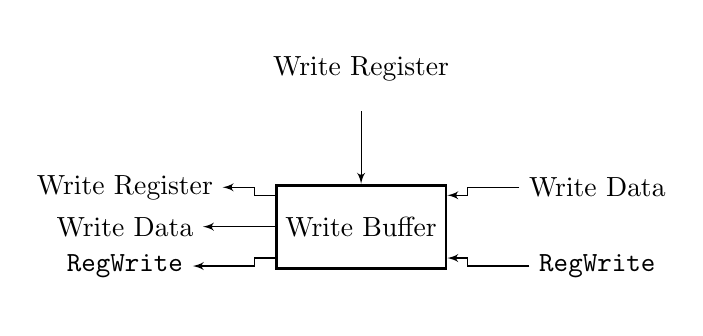
\begin{tikzpicture}
            \node[block] (wb) at (0,0) {Write Buffer};
            \node[empty] (wr) at (0,2) {Write Register};
            \node[empty] (wd) at (3,0.5) {Write Data};
            \node[empty] (rw) at (3,-0.5) {\texttt{RegWrite}};
            \node[empty] (wr2) at (-3, 0.5) {Write Register};
            \node[empty] (wd2) at (-3, 0) {Write Data};
            \node[empty] (rw2) at (-3, -0.5) {\texttt{RegWrite}};

            \path[draw, ->] (wr) -- (wb);
            \path[draw, ->] (wd) -| (1.35, 0.45) |- (wb.20);
            \path[draw, ->] (rw) -| (1.35, -0.45) |- (wb.340);
            \path[draw, ->] (wb) -- (wd2);
            \path[draw, ->] (wb.160) -| (-1.35,0.45) |- (wr2);
            \path[draw, ->] (wb.200) -| (-1.35,-0.45) |- (rw2);
        \end{tikzpicture}
    \end{figure}
\end{frame}
\subsection{Implementation \& Testing}
\begin{frame}
    Implementing the Write Buffer in SME is straightforward. Construct a
    process that holds 3 values, and on each clock, output the values in the
    hold, and store the values from the input.

    \vspace{\baselineskip}
    This is tested in the same matter as the previous components.
\end{frame}

% exit section
\AtBeginSection{}
\section*{}

% {{{ Bibliography ------------------------------------------------------------
%\begin{frame}{Bibliography}
%  \tiny
%  \bibliographystyle{plain}
%  \bibliography{pl}
%\end{frame}
% }}} -------------------------------------------------------------------------

\end{document}
